%*******************************************************************************
% Copyright (c) 2014 Formal Mind GmbH and others
% All rights reserved. This program and the accompanying materials
% are made available under the terms of the Eclipse Public License v1.0
% which accompanies this distribution, and is available at
% http://www.eclipse.org/legal/epl-v10.html
% 
% Contributors:
%     Michael Jastram - initial Copy
%     Maha Jastram - susequent improvements
%******************************************************************************/

\documentclass[twoside,10pt]{book}
\usepackage{float}
\usepackage{graphicx}
\usepackage{hyperref}
\usepackage[utf8]{inputenc}
\usepackage{soul}
\usepackage{wrapfig}
\usepackage{makeidx}
\usepackage[table,xcdraw]{xcolor}

%----------------------------------------------------------------------------------------
%	MACROS
%----------------------------------------------------------------------------------------

\newcommand{\pror}[0]{ProR}

\definecolor{menugray}{RGB}{230,230,230}
\sethlcolor{menugray} 
\newcommand{\menu}[1]{\hl{\texttt{#1}}}
\newcommand{\term}[1]{\textit{#1}}
\newcommand{\eclipsehelp}[2]{\href{http://help.eclipse.org/luna#1}{#2}}
\renewcommand{\floatpagefraction}{.8} % /improves floating of figures

%----------------------------------------------------------------------------------------
%	ENVIRONMENTS
%----------------------------------------------------------------------------------------

\definecolor{color-info}{RGB}{0,0,128} 
\newenvironment{info}{\begin{description}\item[\textcolor{color-info}{Information.}]}{\end{description}}

\definecolor{color-warning}{RGB}{128,0,0} 
\newenvironment{warning}{\begin{description}\item[\textcolor{color-warning}{Warning.}]}{\end{description}}

\newsavebox{\mybox}
\newenvironment{example}
{\noindent\textbf{Example}\newline\begin{lrbox}{\mybox}\begin{minipage}{0.97\textwidth}}
{\end{minipage}\end{lrbox}\fbox{\usebox{\mybox}}\vspace{0.3cm}}

\newenvironment{definition}[1]{\begin{quote}\noindent \textbf{#1.}}{\end{quote}}

%----------------------------------------------------------------------------------------
%	DOCUMENT INFO
%----------------------------------------------------------------------------------------

\title{Eclipse ProR User Guide}
\author{by the RMF Community}
\makeindex

%----------------------------------------------------------------------------------------
%	START DOCUMENT
%----------------------------------------------------------------------------------------

\begin{document}        

\maketitle

\tableofcontents

%%%%%%%%%%%%%%%%%%%%%%%%%%%%%%%%%%%%%%%%%%%%%%%%%%%%%%%%%%%%%%%%%%%%%%%%%%%%%%%%%%%%%%%%%
\chapter{Introduction}

%*******************************************************************************
% Copyright (c) 2014 Formal Mind GmbH and others
% All rights reserved. This program and the accompanying materials
% are made available under the terms of the Eclipse Public License v1.0
% which accompanies this distribution, and is available at
% http://www.eclipse.org/legal/epl-v10.html
% 
% Contributors:
%     Michael Jastram - initial Copy
%******************************************************************************/

The importance of requirements has been recognized for a long time.  And with the advent of computer-aided engineering tools, a number of proprietary solutions popped up all over the place.  While this helped organizations to manage their requirements more efficiently, interoperability became a major issue.

The development of the ReqIF standard for requirements exchange finally provided a standard, feature-rich way of accessing requirements data.  Eclipse was the obvious choice for a reference implementation of this open standard.  The result is the Eclipse Requirements Modeling Framework, a complete, open source, user-friendly implementation of ReqIF.

This handbook is a comprehensive documentation of the \pror{} tool, which is based on Eclipse RMF.  All answers with respect to tool use should be answered here.  Furthermore, it contains a small tutorial (Chapter~\ref{sec:tutorial}) to get you started quickly.

Keep in mind that tools are meant to support processes, not the other way around.  \pror{} is a flexible tool, and it can be tailored to support your processes.  But development processes are explicitly outside the scope of this handbook.

\begin{info}
If you are interested in adopting a lightweight development process that can be used with \pror{}, visit our initiative \href{http://re-teaching.org}{re-teaching.org}.
\end{info}

\section{RMF, ProR, Essentials and formalmind Studio}
\index{formalmind Studio}
\index{ProR Essentials}
\index{Essentials}

There are a few derivatives of the RMF project that may be confusing.  The following will
help you to understand the ecosystem and how the pieces fit together:

\begin{description}
\item[RMF.] The Requirements Modeling Framework (RMF) is an open source project that is managed by the Eclipse Foundation.  It consists of software code, documentation, mailing lists, online forum, etc.
\item[ProR.] ProR is the name of the user interface that allows users to work with ReqIF-based requirements.  ProR is typically installed into existing Eclipse installations.  There used to be a stand-alone build of ProR, which has been discontinued.
\item[RMF Core.] While ProR is the front end of RMF, the Core is the back end.  This distinction is primarily intended for developers.
\item[ProR Essentials.] The company Formal Mind created this collection of add-ons that make ProR much more usable.  For instance, Essentials allow to edit and render formatted text.
\item[formalmind Studio.] As there is no stand-alone version of ProR available, Formal Mind created one, which comes with Essentials preinstalled.  For users who ``just want to edit requirements'', this is the most convenient way of getting started.
\end{description}

\section{Compatibility}

\pror{} and RMF require at least Java 6 and Eclipse 3.8.  The following table elaborates.






%*******************************************************************************
% Copyright (c) 2014 Formal Mind GmbH and others
% All rights reserved. This program and the accompanying materials
% are made available under the terms of the Eclipse Public License v1.0
% which accompanies this distribution, and is available at
% http://www.eclipse.org/legal/epl-v10.html
% 
% Contributors:
%     Michael Jastram - initial Copy
%     Maha Jastram - susequent improvements
%******************************************************************************/

\pror{} is the user interface of the Eclipse Requirements Modeling Framework.  This handbook strives to be a complete reference for \pror{}.  Included is a tutorial making it as easy as possible for new users to get started with requirements engineering.

% ===================================================================================
\section{Conventions}
% ===================================================================================

Throughout this book you'll see the following conventions:

% Formatted like remark
\begin{info}
This is where you'll find useful information or tips.
\end{info}

\begin{warning}
This will mark things to be aware of.
\end{warning}

\begin{example}
Examples will be marked as such.
\end{example}

When referring to \menu{menus} or \menu{user interface elements}, they are marked as shown here.



\section{Improve this Document}
Documentation is one of those things that gets easily neglected in open source projects.
It is also one of the easiest for outsiders to contribute to.  Please refer to
Chapter~\ref{sec:styleguide} if you would like to help improving this user guide.

%*******************************************************************************
% Copyright (c) 2014 Formal Mind GmbH and others
% All rights reserved. This program and the accompanying materials
% are made available under the terms of the Eclipse Public License v1.0
% which accompanies this distribution, and is available at
% http://www.eclipse.org/legal/epl-v10.html
% 
% Contributors:
%     Michael Jastram - initial Copy
%     Maha Jastram - susequent improvements
%******************************************************************************/

% ===================================================================================
\section{Acknowledgements}
% ===================================================================================

Many parties were involved in the creation of RMF.  We would like to thank the core team that made it possible.

\begin{figure}[H]
  \centering
  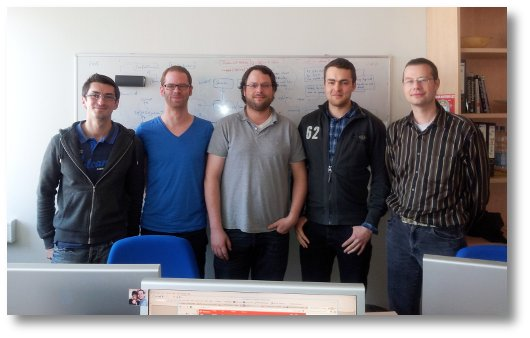
\includegraphics[width=\textwidth]{../rmf-images/2012_03_sprint_team.jpg}
  \caption{The RMF team during a Sprint in April 2012 in Düsseldorf, Germany (left to right) Lukas Ladenberger, Mark Brörkens, Ingo Weigelt, Said Salem, Michael Jastram}
  \label{fig:intro_core_team}
\end{figure}

The roots of this project were created by Andreas Graf, Michael Jastram and Nirmal Sasidharan, who joined together individual projects to create RMF.  Their efforts were financed by the research projects itea Verde and FP7 Deploy.  RMF was assembled at the Eclipse Foundation, where it has been active ever since.  Figure~\ref{fig:intro_core_team} shows four of the five RMF Committers at a joint coding session (missing is Andreas Graf).


%*******************************************************************************
% Copyright (c) 2014 Formal Mind GmbH and others
% All rights reserved. This program and the accompanying materials
% are made available under the terms of the Eclipse Public License v1.0
% which accompanies this distribution, and is available at
% http://www.eclipse.org/legal/epl-v10.html
% 
% Contributors:
%     Michael Jastram - initial Copy
%     Maha Jastram - susequent improvements
%******************************************************************************/

% ===================================================================================
\section{License}
\label{sec:license}
% ===================================================================================

This work, or parts thereof, are licensed under the \href{https://www.eclipse.org/legal/epl-v10.html}{Eclipse Public License Version 1.0} as part of the Eclipse Requirements Modeling Framework (RMF) project at \href{https://www.eclipse.org/rmf}{eclipse.org/rmf}.



%%%%%%%%%%%%%%%%%%%%%%%%%%%%%%%%%%%%%%%%%%%%%%%%%%%%%%%%%%%%%%%%%%%%%%%%%%%%%%%%%%%%%%%%%

%%%%%%%%%%%%%%%%%%%%%%%%%%%%%%%%%%%%%%%%%%%%%%%%%%%%%%%%%%%%%%%%%%%%%%%%%%%%%%%%%%%%%%%%%
\chapter{Overview}
\label{sec:overview}
This chapter provides a high-level overview of requirements engineering, requirements tooling, ReqIF and the terminology.

% ===================================================================================
\section{Requirements Engineering \& Management}
\label{sec:requirements_engineering}
\index{requirements engineering}
% ===================================================================================

This book is concerned with \pror{} a tool for requirements engineering.

\begin{definition}[Requirements Engineering]
\index{requirements engineering}
``Requirements engineering (RE) refers to the process of formulating, documenting and maintaining software requirements'' (\href{http://en.wikipedia.org/wiki/Requirements_engineering}{Wikipedia}).

We'd argue that RE also includes \textit{system} requirements.  Further, requirements are typically unstructured natural language.  Of high interest these days is model-driven requirements engineering.
\end{definition}

But engineering the requirements is not enough: they need to be \textit{managed}.

\begin{definition}[Requirements Management]
\index{requirements management}
``Requirements management is the process of documenting, analyzing, tracing, prioritizing and agreeing on requirements and then controlling change and communicating to relevant stakeholders. It is a continuous process throughout a project.''
\end{definition}

% ===================================================================================
\section{Tools}
\label{sec:re-tools}
\index{tools}
% ===================================================================================

There are many tools available for requirements engineering.  These include free or cheap ones, like Microsoft Word and Excel, Wikis and issue trackers.  There are expensive, professional ones available, like IBM Rational DOORS, PTC Integrity or Visure IRQA.  Lately, there are also web-based tools, like Polarion.

\pror{} falls into the category of free tools.  But compared to the ones mentioned, it contains important features from professional tools, including traceability and typed attributes.  Further, by taking advantage of the Eclipse ecosystem, the tool can be augmented by plug-ins for version support, model integration, and much more.

\begin{info}
  Professional support, commercial components and integration services are available from \href{http://formalmind.com}{Formal Mind} and other service providers.
\end{info}


% ===================================================================================
\section{Requirements Interchange Format (ReqIF)}
\label{sec:reqif}
\index{ReqIF}
\index{Requirements Interchange Format}
% ===================================================================================

ReqIF stands for Requirements Interchange Format.  It is an exchange format for requirements and a data model.  \pror{} is an editor that can directly view and modify ReqIF data.

ReqIF was created to support the exchange of requirements across organizations.  For instance, it allows a manufacturer to send requirements to suppliers.  The suppliers can then comment and review the requirements, or they can create a system specification that is linked to the requirements.

ReqIF is an (\href{http://www.omg.org/spec/ReqIF/}{official OMG standard}).

\begin{warning}
ReqIF uses its own terminology.  Section~\ref{sec:terminology} defines the ReqIF vocabulary and how it relates to the terms used in classical requirements engineering.
\end{warning}

% -----------------------------------------------------------------------------------
\subsection{ReqIF History}
\label{sec:history}
\index{history}
% -----------------------------------------------------------------------------------

For technical and organizational reasons, two companies in the manufacturing industry are rarely able to work on the same requirements repository and sometimes do not work with the same requirements authoring tools.  A generic, non-proprietary format for requirements information is required to cross the chasm and to satisfy the urgent industry need for exchanging requirement information between different companies without losing the advantage of requirements management at the organizations' borders.

The Requirements Interchange Format (ReqIF) described in this RFC defines such a tool-independent exchange format.  Requirement information is exchanged by transferring XML documents that comply to the ReqIF format.

In 2004, the HIS (Hersteller Initiative Software), a panel of Germany's automotive manufacturers (Daimler, VW, Porsche, Audi and BMW Group) developed the idea of creating the ``Requirements Interchange Format''.  In 2005, the first version of that format was presented at the REConf®, a conference about requirements engineering and management, in Munich.  In 2008, the HIS Steering Committee decided that the internationalization and maintenance of the Requirements Interchange Format should be proceeded with the ProSTEP iViP Association.  A project was set up and a team was built that includes members of the ProSTEP iViP Association, representatives of manufacturing companies (Audi, BMW  Group, Daimler, VW, Bosch and Continental), tool vendors (Atego, IBM, MKS) and development partners (HOOD GmbH, PROSTEP AG).

\begin{info}
Further reading: \href{http://formalmind.com/de/blog/his-exchange-process-requirements-all-you-ever-wanted-know}{The HIS Exchange Process for Requirements–all you ever wanted to know}.
\end{info}

The ReqIF team expects that making the Requirements Interchange Format an OMG standard increases the number of interoperable exchange tool implementations on the market, fosters the trust of companies exchanging requirement information in the exchange format and provides safety of investments to tool vendors.

% -----------------------------------------------------------------------------------
\subsection{Previous Versions of ReqIF}
\index{RIF}
\label{sec:RIF}
% -----------------------------------------------------------------------------------

This document is submitted as RFC of the Requirements Interchange Format (ReqIF) to the OMG.  Before the submission, the Requirements Interchange Format has been a specification proposed by the HIS and in its latest version, a recommendation of ProSTEP iViP.  For these versions, the abbreviation ``RIF'' has been applied.  The HIS released the Requirements Interchange Format as RIF 1.0, RIF1.0a, RIF 1.1; RIF1.1a and the ProSTEP iViP released the recommendation RIF 1.2.

As the acronym RIF has an ambiguous meaning within the OMG, the acronym ReqIF has been introduced to separate it from the W3C`s Rule Interchange Format.  ReqIF 1.0 is the direct successor of the ProSTEP iViP recommendation RIF 1.2.

\begin{warning}
The ProR GUI does currently not support RIF.
\end{warning}

% -----------------------------------------------------------------------------------
\subsection{Internal Attributes}
\label{sec:reqif_internal_attributes}
\index{internal attributes}
\index{attributes!internal}
% -----------------------------------------------------------------------------------

ReqIF allows users to define the attributes that SpecObjects may carry.  In addition to these, there are a number of internal attributes that are defined by the ReqIF standard.  Examples include an internal ID, or the last change timestamp.

These internal attributes are rarely of interest to users who just want to work with requirements.  However, they may be of interest to tool experts, or may be inspected for troubleshooting.

Internal attributes can be accessed from the Properties View, using the \menu{All Attributes} tab.

% ===================================================================================
\section{Terminology}
\label{sec:terminology}
\index{Terminology}
% ===================================================================================

Working with \pror{} can be confusing, as it uses the terminology from ReqIF.  For instance, ReqIF uses \textit{SpecObject}s, rather than \textit{requirements}.  In the following, we define the more important terms.  More terms are defined throughout the document.  You can use the index to find the definition of terms.

\begin{info}
This book uses ReqIF terminology throughout.  Please refer to this chapter to understand the meaning of these terms.
\end{info}





%%%%%%%%%%%%%%%%%%%%%%%%%%%%%%%%%%%%%%%%%%%%%%%%%%%%%%%%%%%%%%%%%%%%%%%%%%%%%%%%%%%%%%%%%

%%%%%%%%%%%%%%%%%%%%%%%%%%%%%%%%%%%%%%%%%%%%%%%%%%%%%%%%%%%%%%%%%%%%%%%%%%%%%%%%%%%%%%%%%
\chapter{Tutorial}
\label{sec:tutorial}
\section{Basic ReqIF Concepts}

A ReqIF model is a structured collection of natural language
requirements. However, it comes with its own terminology. For instance,
a ``Requirement'' is called ``SpecObject'' in ReqIF:

A ReqIF model has some similarities to a Excel Spreadsheet, although
there are some notable differences. It's simply meant as a starting
point to get a feel for ReqIF.

The following table compares a Spreadsheet model with a ReqIF model,
introduces the terminology and explains it:

\begin{description}
  \item[Specification.] (Excel-equivalent: Sheet)  A ReqIF model
consists of an arbitrary number of Specifications. The Specification is
the ``Container'' for the Requirements. Think of an Excel Document, that
allows you to create an arbitrary number of Sheets. There are two
differences to Excel: (1) The requirements in the Specification are
references (which means that the same requirement can appear in multiple
places); (2) The content of Specification is hierarchical.

  \item[SpecObject.] (Excel-equivalent: Row) A SpecObject represents the actual
Requirement. A requirement typically has a number Attributes. Again
compared with Excel, each row in a Sheet represents a requirement. In
contrast to Excel, the ReqIF model may contain SpecObjects that do not
appear in any Specification (whether this is useful is a different
question).

  \item[Attribute.] (Excel-equivalent: Cell) Besides the actual text of the
requirement, typical Attributes include ID, Status, etc. Note that there
are no ``standard'' Attributes. The ReqIF model contains the definitions
of the Attributes. Here the Excel analogy starts to break down. In
Excel, each row has the same columns. Different SpecObjects may have
different sets of Attributes.

  \item[SpecType.] (Excel-equivalent: Column configuration) Each SpecObject
has a SpecObjectType. The SpecObjectType contains a list of Attributes
for the SpecObject. For instance, the SpecObjectType ``Headline'' may
have only one Attribute ``HeadlineText''. Another SpecObjectType
``Requirement'' may have three Attributes, ``ID'', ``Description'' and
``Status''. A Specification may then contain a mixture of SpecObjects
with different types.

\end{description}

There are many more concepts, but this is enough to get us started.

Let's look at a concrete example to understand this. Here is a snippet
of a Specification:

The table shows the first four SpecObjects, as visualized in a
Specification. The tree-like structure is recognizable: INF-1 is a node
with three children, REQ-1, REQ-2 and REQ-3 (this can be seen by the
indentation). Let's look at INF-1 and REQ-1. If they would be selected
in the GUI, the Property pane would show their Attributes, as it is
shown to the right.

INF-1 has two attributes, ``Description'' and ``ID''. The SpecObjectType
is ``Information Type'' (shown as the root in the properties view).

REQ-1 has three attributes, ``Description'', ``ID'' and ``Status''. The
SpecObjectType is called ``Requirements Type''. Let's have a closer look
at that one.

The ``Requirements Type'' SpecObjectType is shown in the picture, with
arrows indicating how the Attributes relate to the SpecObjectType (a
simple one-to-one relationship). A SpecObjectType has one entry for each
Attribute, consisting of a name and a Datatype. For instance, the first
entry has the name ``ID'' and the datatype ``T\_ID\_REQ''. Note that
multiple Attributes may have the same Datatype: ``Description'' and
``Status'' both have the Datatype ``T\_String32k''.

Last, The Datatypes must be defined as well. In this example, there are
two Datatypes, ``T\_String32'' and ``T\_ID\_REQ''. These are finally
based on a number of standard types that ReqIF supports.

NOTE: As of this writing, we only implemented the simple and the
enumeration ReqIF types. This leaves out the complex ones (rich text,
attachments, embedded files, etc.) for now.

\section{Tutorial 1: Creating a basic ReqIF Model}

In this Section, we will build a ReqIF model from scratch, step by step.

\subsection{Install \pror{}}

You can download \pror{} from the
\href{http://www.eclipse.org/rmf/download.php}{Download page}.
Alternatively, you can install \pror{} in any Eclipse-Installation via its
update site (also listed on the
\href{http://www.eclipse.org/rmf/download.php}{Download page}). Using
the update site allows you to use the Eclipse Update mechanism,
something that is currently not yet enabled for the standalone version.

\subsection{Create the Model}

\begin{itemize}

\item
  Make sure that you have at least one Project in the Workspace;
\item
  Select File \textgreater{} New \textgreater{} Reqif10 Model;
\item
  Select a Project and name the file (ending in .reqif), then click
  ``Finish'';
\item
  In the Window named ``file.reqif'', double-click on ``Requirements
  Document'' button in the ``Specifications'' panel.
\end{itemize}

After this, your window should look more or less as follows:

\begin{figure}[h!]
  \centering
  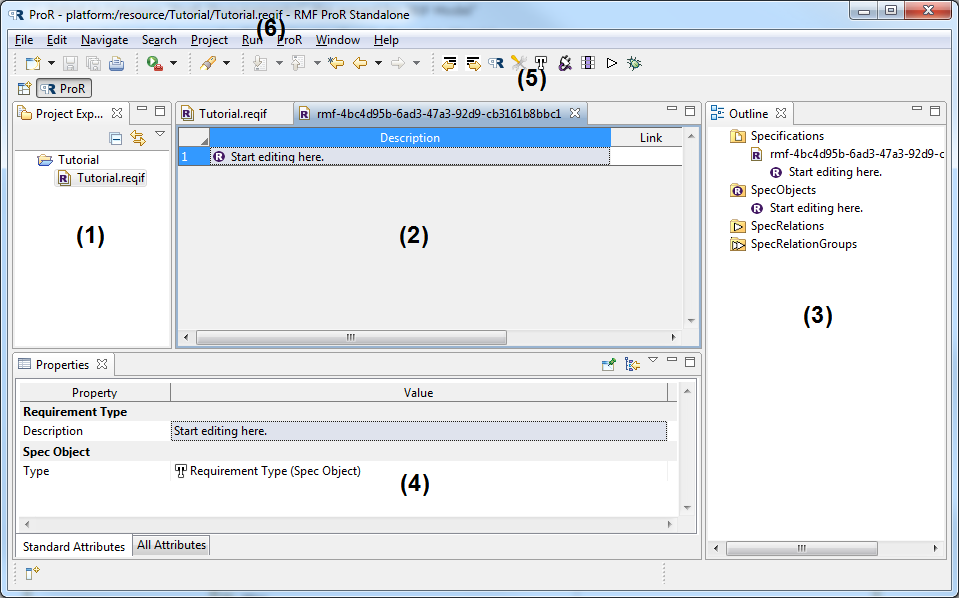
\includegraphics[width=\linewidth]{../rmf-images/pror-screenshot.png}
  \caption{The \pror{} user interface}
  \label{fig:user_interface_overview}
\end{figure}

You will see your ReqIF file in the (1) Project Explorer or the regular
Navigator.

The Editor (2) shows your Specifications.

In the Editor, you see the SpecObjects that exist in this Specification.
There is currently only one, with the description ``Start Editing''.

The Outline (3) has three folders:

\begin{itemize}

\item
  ``Specifications'' shows the Specifications in the ReqIF. You can
  expand the tree to expose the hierarchy of SpecObjects in the
  Specification.
\item
  ``SpecObjects'' shows all SpecObjects in the ReqIF as a flat list.
  Keep in mind that SpecObjects in Specifications are references. In
  contrast, this folder shows all SpecObjects in the ReqIF model, no
  matter whether they appear in any Specification.
\item
  ``SpecRelations'' shows all SpecRelations in the ReqIF as a flat list.
  For now, we will ignore SpecRelations.
\end{itemize}

The properties of a selected Element are shown in the Properties view
(4). As the only Requirement in the model is selected, we see its
SpecObjectType (``Requirements Type'') and its only Attribute
(``Description'') with the value ``Start editing here.''. There are two
tabs ``Standard Attributes'' and ``All Attributes'' at the bottom of the
Properties view. The ``Standard Attributes'' tab shows you all standard
attributes of the selected element. The ``All Attributes'' shows all
existing ReqIF attributes of the selected element.

When a ReqIF Editor is active, there are also additional tool bar items
(5) and an additional menu (6).

\subsection{Customizing the SpecType}

To get familiar with the system, next we will:

\begin{itemize}

\item
  Add two more attributes to the SpecObjectType called ``ID'' and
  ``Owner''
\item
  We will show those Attributes in the Specification
\end{itemize}

To add new attributes, we open the Datatype Configuration dialog with
\pror{} \textgreater{} Datatype Configuration.

The resulting Dialog has a folder for SpecTypes and Datatypes.
Currently, there is only one Datatype (T\_String32k) and two SpecTypes,
one called ``Requirements Type'' with one Attribute ``Description'' and
one called ``Specification Type'' with one Attribute ``Description''.

We add more Attributes to ``Requirements Type'' by right-clicking
``Requirements Type'' and selecting ``New Child \textgreater{} Attribute
Definition String''. This will create a new element. Upon selecting, we
can rename it in the lower pane. We do this twice for ``ID'' and
``Owner''. We assign both Attributes the same Datatype,
``T\_String32k''. In the end, the dialog should look as follows:

\begin{figure}[h!]
\centering
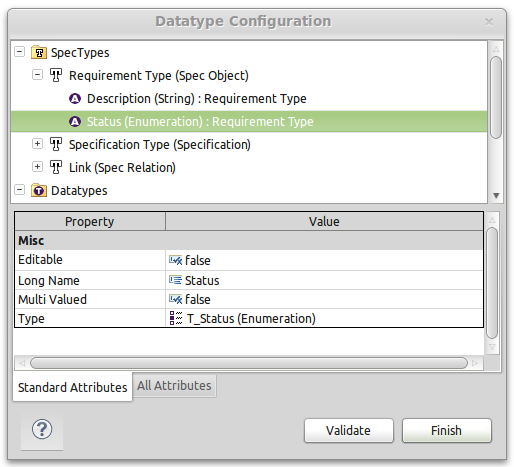
\includegraphics[width=0.8\linewidth]{../rmf-images/pror_datatype_configuration.png}
\caption{Datatype Configuration Dialog}
\label{fig:datatype_configuration}
\end{figure}

Upon closing the dialog, little will have changed - the Specification
still shows just two columns, Description and Link. However, if you
select the requirement, you will see the new Properties (ID and Owner)
in the Property view.

\subsection{Showing the new Attributes in the Specification}

To show the new Attributes in the Specification, we have to configure
the Specification columns. We do this by selecting \pror{} \textgreater{}
Column Configuration.

The resulting Dialog shows one entry for the one and only Column of the
Specification. By clicking on the ``Add Column'' icon at the top of the
dialog, we can add two more columns. We do this and name them ``ID'' and
``Description'' (in the lower pane). Feel free to rearrange the order
with drag and drop, as you see fit. When all is done, the dialog should
look as follows:

\begin{figure}[h!]
\centering      
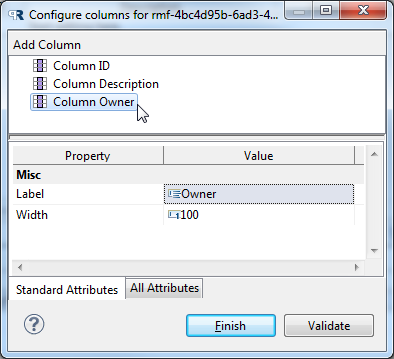
\includegraphics[width=0.8\linewidth]{../rmf-images/pror_column_configuration.png}      
\caption{Column Configuration}
\label{fig:column_configuration}
\end{figure}

Note that you have to provide Strings for the columns for the same
reason that we used Strings for the Labels earlier: This way we can
easily match multiple SpecObjects of different types.

You can actually adjust the width of the columns simply by dragging the
column headers.

\subsection{Adding new SpecObjects}

Now we can finally add SpecObjects by right-clicking on a row in the
Specification. In the context-menu, there are two submenus: ``New
Child'' and ``New Sibling''. ``New Child'' is the only way to produce a
hierarchical structure.

In both menus, there are three entries ``Spec Hierarchy'', ``Adding
SpecObjects'' and ``SpecObject (Requirement Type)''. Some background is
needed here:

We said before that Specifications contain references to SpecObjects. A
SpecHierarchy is the ``Wrapper'' that allows the hierarchical structure
and that points to the referred SpecObject. Usually, we don't have to be
concerned with them. Therefore the second option: If selected, a new
SpecHierarchy is created and associated with a new SpecObject, which in
turn is set immediately to the given SpecObjectType. If we had more than
just one SpecObjectType (besides ``Requirements Type''), there would be
an entry for each type in the context menu.

To continue the exercise, select the child ``SpecObject (Requirement
Type)''. Now we have two SpecObjects. Create a few more values and enter
some values. You can edit directly in the Specification, as you would in
Excel. Play around with Hierarchies.

You can drag and drop SpecObjects as a sibling or as a children. The
highlighting feedback helps you to find out whenever you shifting a
SpecObject as sibling or as a children. For instance, if you are
dragging a SpecObject over another one, the entire cell will be
highlighted. This means, that the SpecObject will be assigned as a
children to the dropped SpecObject.

\begin{figure}[h!]
\centering
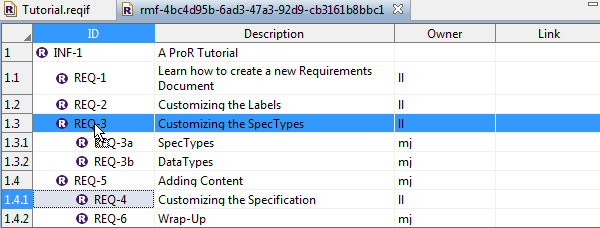
\includegraphics[width=\linewidth]{../rmf-images/feedback1.png}      
\caption{Drag and Drop as Child Object}      
\label{fig:dragAndDropChild}
\end{figure}

If you are dragging a SpecObject between two rows, you get also a visual
feedback an the SpecObject will be assigned as sibling:

\begin{figure}[h!]
\centering      
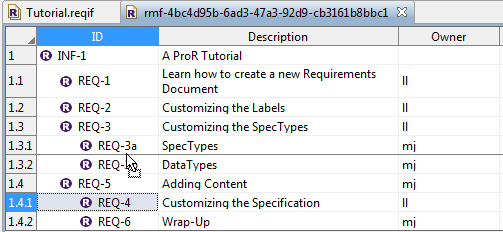
\includegraphics[width=0.8\linewidth]{../rmf-images/feedback2.png}      
\caption{Drag And Drop as Sibling Object}      
\label{fig:dragAndDropSibling}
\end{figure}

After some playing around, our Specification may look like this:

\begin{figure}[h!]
\centering      
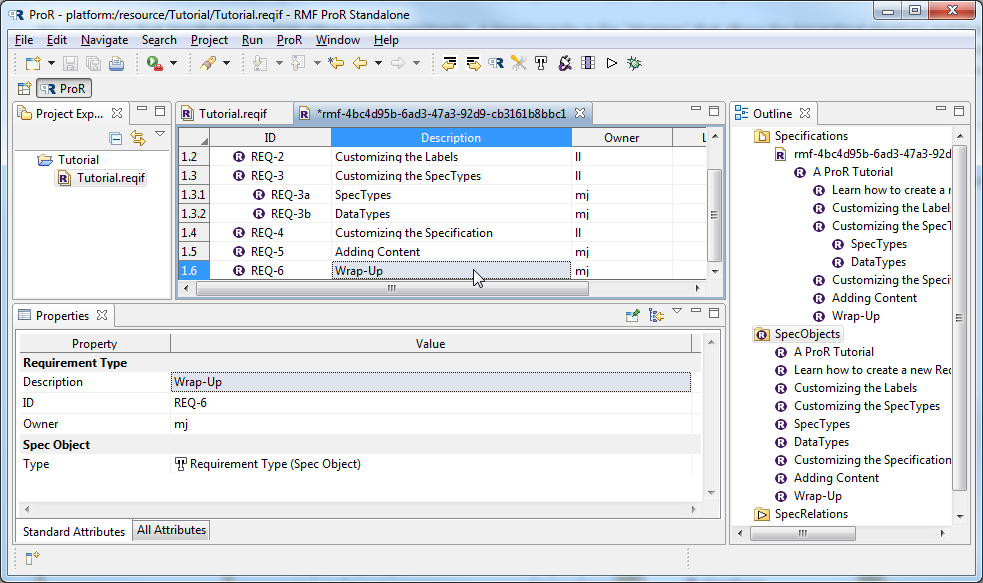
\includegraphics[width=\linewidth]{../rmf-images/pror_speceditor_2.png}      
\caption{Improved Specification}      
\label{fig:improvedSpec}
\end{figure}

\subsection{Export Specification as HTML}

If you want to export your Specification as HTML, go to ``File'' in the
main menu and click ``Print...''. The HTML representation is generated
and automatically opened in your default browser.

\subsection{Conclusion}

Quite an achievement - but also quite a bit of work to get started.
Also, entering information requires a lot of clicking, and some of the
descriptions are not completely visible. In the next part of the
tutorial, we will address these issues.

\section{Tutorial 2: Use Presentations}

We will continue where we left off with Tutorial 1 and we assume that
you have \pror{} in front of you with a similar model.

In this tutorial we will introduce Presentations. Presentations are
Eclipse Plug-Ins that extend the functionality of \pror{}. Specifically:

\begin{itemize}
\item
  Presentations can change the way how Attributes are rendered in the
  Specification
\item
  Presentations can change the way how Attributes are edited in the
  Specification
\item
  Presentations can perform tasks in the background.
\end{itemize}

\pror{} comes with a number of standard presentations that we will
introduce in this tutorial.

\subsection{Linewrap Presentation}

By default, text is not wrapped in cells. We will enable the Linewrap
Presentation for the Description column.

To do this, we select \pror{} \textgreater{} Presentation Configuration.

The dialog shown has no entries. The drop-down menu ``Select Action...''
at the top allows us to create new Presentations. We select the
``Linewrap'' Presentation. This will create a new entry in the upper
pane. Upon selecting it, we can configure it in the lower pane.

A Linewrap Presentation has only one configuration element, the
Datatype. We select ``T\_String32k''. This means that from now on, all
Attributes of this type will be rendered with the Linewrap Presentation.
Upon completion, the dialog should look like this:

\begin{figure}[h!]
\centering
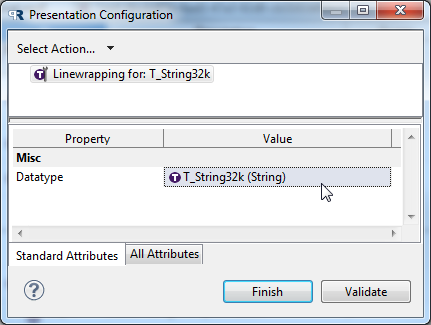
\includegraphics[width=0.8\linewidth]{../rmf-images/pror_presentation_configuration.png}      
\caption{Presentation Configuration Dialog}      
\label{fig:presentationConfig}
\end{figure}

Upon closing the dialog, the lines that are too long should be wrapped
automatically. Also, upon clicking on a cell, the content is now wrapped
in the editor.

\subsection{ID Presentation}

It would be nice if every SpecObject had its own unique ID. Actually, it
does (it is shown in the Property View, if a SpecObject is selected in
the Outline View). But that ID is meant for machines and is not
practical.

The ID Presentation allows the automatic creation of IDs. Let's create
one.

Remember that Presentations are associated with Datatypes, not
Attributes. Thus, we first have to create a new Datatype. We then
associate that Datatype with the Attribute ``ID''. We described this
process in the first tutorial. Here is a screen-shot of the
configuration dialog, when all is done:

\begin{figure}[h!]
\centering      
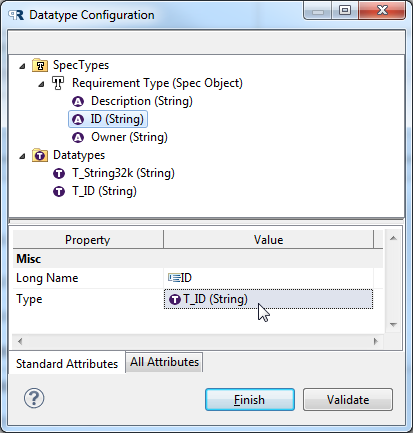
\includegraphics[width=0.8\linewidth]{../rmf-images/pror_id_configuration.png}      
\caption{Datatype Configuration Dialog}      
\label{fig:datatypeConfig}
\end{figure}

The last step is, like before, to associate that Datatype with the
Presentation.

We open the Presentation Configuration and create a new Presentation
from the dropdown menu ``Select Action...'', this time of type ``Id''
Presentation. We associate it with the newly created Datatype. After
configuration, the dialog should look as follows:

\begin{figure}[h!]
\centering      
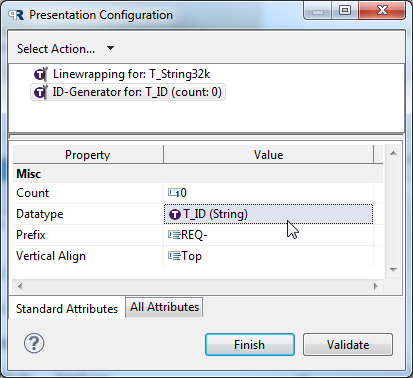
\includegraphics[width=0.8\linewidth]{../rmf-images/pror_id_presentation.png}      
\caption{ID Configuration Detail}      
\label{fig:idConfig}
\end{figure}

Note that you could adjust the prefix and the Count.

NOTE: At this point, the Presentation doesn't check yet for duplicates.
It simply grabs a new value from count, increments it and uses it. Also,
existing values are not overwritten.

\section{Tutorial 3: Advanced SpecTypes}

So far, we have a model with only one SpecObjectType. In this tutorial,
we will show how we can work with multiple SpecTypes, and we will
introduce other SpecTypes.

\subsection{Multiple SpecTypes}

The first entry in our Specification (``A \pror{} Tutorial'') isn't really
a requirement. Thus, it doesn't need an ID or an owner, and it would be
nice to Highlight it somehow. For Highlighting, we have the Headline
Presentation. We will:

\begin{itemize}

\item
  Create a new ``Headline'' SpecObjectType
\item
  Create a new Datatype that will be used for the Headline content
\item
  Associate that Datatype with the Headline Presentation
\end{itemize}

With \pror{} \textgreater{} Datatype Configuration we get the Dialog where
we can create new SpecTypes and Datatypes. For the first time, we create
a new SpecObjectType by right-clicking on ``SpecTypes''. One of the
entries in the child menu is ``SpecObject Type''.

Once created, we select it and rename to ``Headline Type'' it in the
properties.

Then we give it a new Attribute called ``Description''.

NOTE: It is important that we call it description. This matches the
Attribute from ``Requirement Type''. By using the same name, we ensure
that the Attributes appear in the same column, even though they are
different Attributes.

We do not set the type yet, as we need to create a new one. We do this
by right-clicking on ``Datatypes''. There we create a new ``Datatype
Definition String'' and call it ``T\_Headline''. Now we can go back to
the Description Attribute and set the type to T\_Headline.

When all this is done, the configuration should look like this:

\begin{figure}[h!]
\centering      
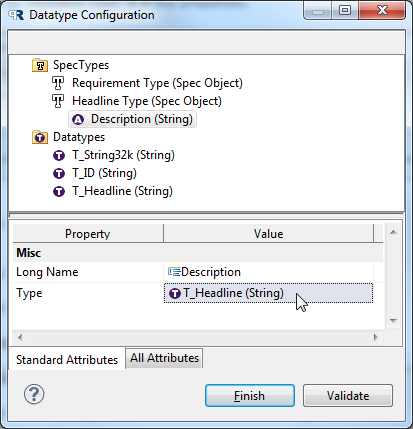
\includegraphics[width=0.8\linewidth]{../rmf-images/pror_datatype_headline1.png}      
\caption{Datatype Configuration for the Headline Presentation}      
\label{fig:headlineConfig}
\end{figure}

You can change the type of a SpecObject by selecting it an changing it
in the Properties view. Please note that currently all existing values
are lost when changing the type.

After the changes, the GUI should look as follows:

\begin{figure}[h!]
\centering      
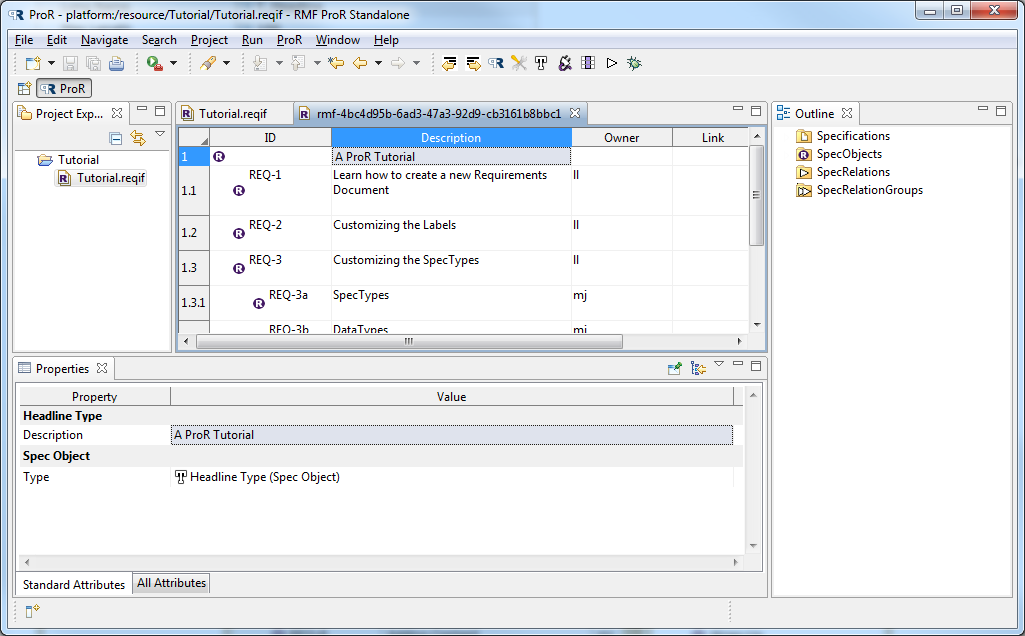
\includegraphics[width=\linewidth]{../rmf-images/pror_gui_with_headline.png}      
\caption{Activated Headline Configuration}      
\label{fig:activeHeadlineConfig}
\end{figure}

Note the following:

\begin{itemize}
\item
  The columns ``ID'' and ``Owner'' are now empty and cannot be edited
  for the Headline
\item
  Note how the Property View changes, as you select SpecObjects of
  different types
\item
  Right-clicking on a row now shows one more option for child/sibling
  creation: A new entry of type ``Headline Type''
\end{itemize}

Last, we will use the Headline Presentation for the type T\_Headline.
This is done via the Presentation Configuration, and should result in
the following. In addition, you can change the font size of the headline
in the ``Size'' Attribute:

\begin{figure}[h!]
\centering      
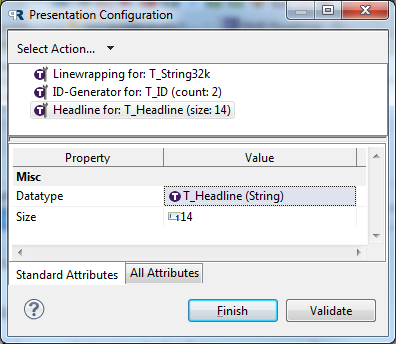
\includegraphics[width=0.8\linewidth]{../rmf-images/pror_datatype_headline2.png}      
\caption{Presentation Configuration for Headline}      
\label{fig:headlineConfig2}
\end{figure}

\subsection{Other SpecTypes}

You may have noticed in the Datatype Configuration Dialog, that
right-clicking on ``SpecTypes'' offered more options, besides ``Spec
Object Type''. A number of ReqIF-Elements can have Attributes.

We will now create a ``Specification Type'' and assign it to our
Specification.

Try to create a ``Specification Type'' and configure it as shown in the
screenshot:

\begin{figure}[h!]
\centering      
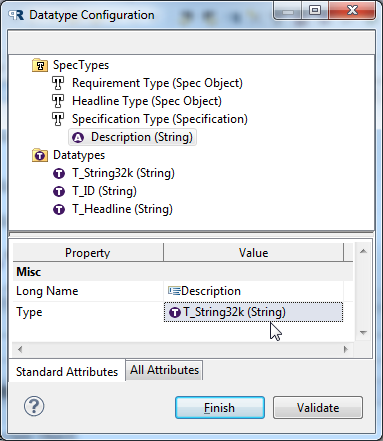
\includegraphics[width=0.8\linewidth]{../rmf-images/pror_new_spectype.png}      
\caption{Creating a New SpecType}      
\label{fig:newSpecType}
\end{figure}

Next, we will assign this type to the one Specification that we have. To
do this we select the Specification in the Outline View. That will show
the Specification's Properties in the Properties View. The ``Type''
Property is empty. We select ``Specification Type'' from the drop down.
As soon as it is selected, the Attribute ``Description'' will appear in
the properties view.

\section{Tutorial 4: Links between SpecObjects (SpecRelations)}

The implementation of SpecRelations is not complete yet. Still here are
a few pointers to show what is planned.

\subsection{Creating SpecRelations}

SpecRelations are created by ``Link-Dragging''. This is platform
specific:

\begin{itemize}

\item
  Linux: Dragging with Ctrl-Shift
\item
  Mac: ???
\item
  Windows: Dragging with Alt
\end{itemize}

Showing links as children can be switched on or off with the little
triangle icon in the toolbar:

\begin{figure}[h!]
\centering      
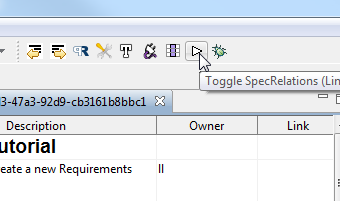
\includegraphics[width=0.8\linewidth]{../rmf-images/pror_toggle_links.png}      
\caption{Toggle Links on and off}      
\label{fig:toggleLinks}
\end{figure}

After creating a link:

\begin{itemize}
\item
  The ``Link'' column shows incoming and outgoing links
\item
  The SpecRelations are shown as children in the Specification view
\end{itemize}

SpecRelations can have their own Types. Once a type is set, the
corresponding columns in the Specification are rendered using
Presentations, etc. However. the Type has to be set explicitly (a link
created with dragging has currently no Type).

Here is a Screenshot of a Specification with some Links and a
SpecRelationType that includes a ``Description'' Attribute:

\begin{figure}[h!]      
\centering      
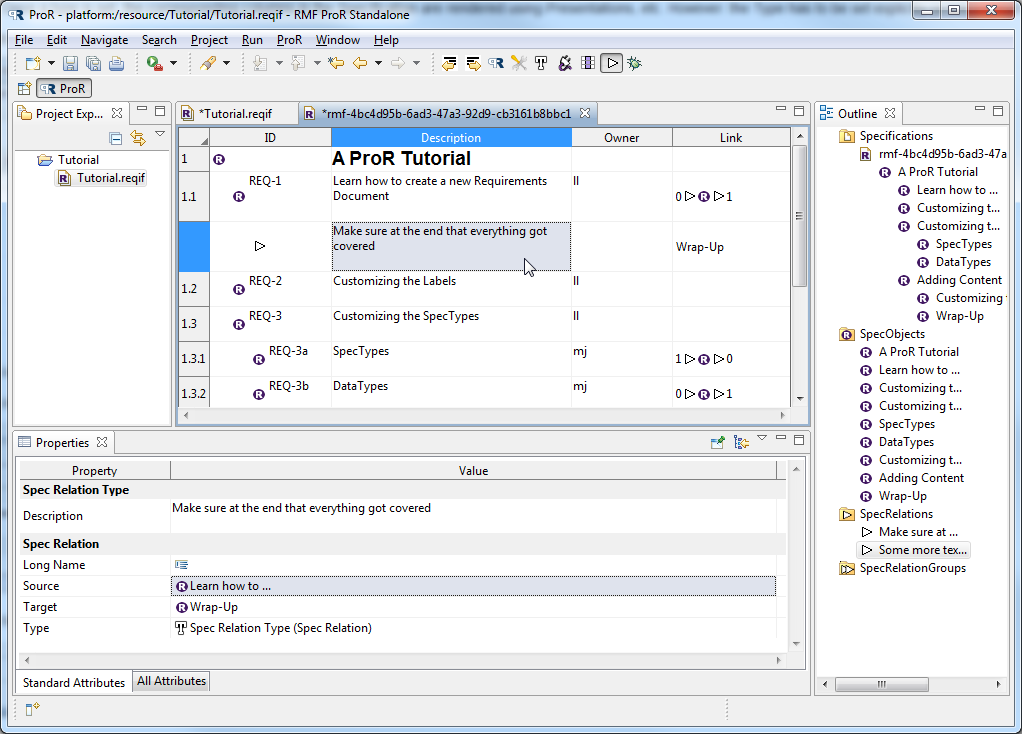
\includegraphics[width=\linewidth]{../rmf-images/pror_gui_with_links.png}      
\caption{Showing Links in the GUI}      
\label{fig:linksInGui}
\end{figure}

Note the following:

\begin{itemize}
\item
  The right column shows incoming and outgoing links
\item
  The number to the left of the triangle is incoming links, the other
  outgoing links
\item
  The outgoing link from REQ-1 is shown
\item
  The link from REQ-1 has a description, and it shows the destination
  name in the ``Link'' column
\end{itemize}

\subsection{Outline View}

Note that the Outline shows a folder with all SpecRelations.


%%%%%%%%%%%%%%%%%%%%%%%%%%%%%%%%%%%%%%%%%%%%%%%%%%%%%%%%%%%%%%%%%%%%%%%%%%%%%%%%%%%%%%%%%

%%%%%%%%%%%%%%%%%%%%%%%%%%%%%%%%%%%%%%%%%%%%%%%%%%%%%%%%%%%%%%%%%%%%%%%%%%%%%%%%%%%%%%%%%
\chapter{Reference}

\pror{} is a desktop application that is based on Eclipse for systems engineering in general, and requirements engineering in particular.

%*******************************************************************************
% Copyright (c) 2014 Formal Mind GmbH and others
% All rights reserved. This program and the accompanying materials
% are made available under the terms of the Eclipse Public License v1.0
% which accompanies this distribution, and is available at
% http://www.eclipse.org/legal/epl-v10.html
% 
% Contributors:
%     Michael Jastram - initial Copy
%     Maha Jastram - susequent improvements
%******************************************************************************/

% ===================================================================================
\section{Eclipse}
\label{sec:eclipse}
% ===================================================================================

\pror{} is an extension of the generic Eclipse Platform.  The following is concerned with Eclipse in general.

\begin{info}
Please consult the 
\eclipsehelp{/topic/org.eclipse.platform.doc.user/gettingStarted/intro/overview.htm?cp=0_0}{Eclipse platform overview} for further information.
\end{info}

% -----------------------------------------------------------------------------------
\subsection{Prerequisites}
% -----------------------------------------------------------------------------------

Eclipse is a Java-based application.  You need a Java Runtime Environment (JRE) on your computer in order to run \pror{}.

\pror{} requires JRE 1.6 or better.  However, some of the features from Essentials require JRE 1.7 or better.  Further, we recommend the version from Oracle, and not OpenJDK.

\begin{info}
You can download Java at \href{https://www.java.com}{java.com}.
\end{info}

% -----------------------------------------------------------------------------------
\subsection{Installation}
\label{sec:installation}
\index{installation}
% -----------------------------------------------------------------------------------

This chapter explores the installation of \term{Eclipse Products}, i.e. software that you can download and run on your computer.  This is in contrast to \term{features} or \term{plugins}, which can be added to an existing product.

When working with Eclipse, you have to start with a base installation.  However, we recommend using \href{https://reqif.academy}{ReqIF Studio}, but you can start with any Eclipse product.

Once you have identified the product you would like to use, you need to download it, which is typically a .zip file.  Create a folder and extract the content of the .zip file into that folder.

\begin{info}
We recommend to call the folder \menu{studio} and to store it where your executables are located: On Windows in \menu{Program Files}, on Linux in \menu{~/bin}.  But any location will do.

We recommend to creating a shortcut for launching it.
\end{info}

You launch the product by double-clicking on the launcher in the folder you created.  For \pror{}, this is called \menu{studio.exe} or \menu{studio}.

The first time you launch Eclipse, it will ask you for the \term{Workspace} location, see Section \ref{sec:workspaces}.

% -----------------------------------------------------------------------------------
\subsection{Updates}
\label{sec:update}
\index{updating}
\index{updates}
% -----------------------------------------------------------------------------------

The Eclipse Update Manager regularly checks for new versions and alerts the user if one is found.  It can also be started manually via \menu{Help | Check for Updates}.

% -----------------------------------------------------------------------------------
\subsection{Installing New Features}
\label{sec:install-add-on}
% -----------------------------------------------------------------------------------

Before you start installing new features, you typically need to connect with the update site that is hosting the feature to be installed.

\begin{definition}{Update Site}
\index{update site}
An update site is a machine-readable URL that allows \pror{} to install new functionality.  Note that visiting the update site with a web browser rarely produces anything meaningful.
\end{definition}

To install a new feature, follow these steps:

\begin{itemize}
\item Open the installation dialog via \menu{Help | Install new Software...}.
\item In the \menu{Work with:} dropbox, either paste the Update Site URL, or select it from the drop down, if you have used it before.  Note that some popular update site URLs may already be preinstalled.
\item Upon selecting an update site, you will see a list of components available from that update site.  Note the checkboxes below that may result in some entries being hidden.  In particular, some update sites do not categorize.  Unchecking \menu{Group items by category} may unveil hidden entries.
\item Click \menu{Next >}.  If all dependencies can be resolved, details about the installation are shown.  Otherwise you have to troubleshoot dependencies (an unthankful job!).
\item Click \menu{Next >}, review and accept the license.
\item Click \menu{Finish}.  If the component has not been digitally signed, you will receive a warning, which you can typically ignore.
\item It is recommended to restart after the installation.
\end{itemize}

\index{unsigned content}
\index{signed content}
\begin{info}
\textbf{Signatures on Content.}  In this day and age, security is obviously very important, particularly for content downloaded from the Internet.  But note that signing is not enough: content must be signed with a trusted, non-expired signature.

Eclipse content should be signed by eclipse.org.  Especially small project release plug-ins that are not signed, reasoning that to a user, a self-signed signature is as good (or bad) as a missing signature.

Ultimately, you need to decide for yourself whether you are willing to run unsigned and/or untrusted content.
\end{info}

% -----------------------------------------------------------------------------------
\subsection{Workspaces}
\label{sec:workspaces}
% -----------------------------------------------------------------------------------

The workspace is a folder on your computer, where all information related to \pror{} is stored.  This includes all your ReqIF files, organized into projects, as well as various meta data.

\begin{info}
Read more about the \eclipsehelp{/topic/org.eclipse.platform.doc.user/gettingStarted/qs-02a.htm?cp=0_1_0_0}{The Workbench} in the Eclipse documentation.

Also, it is possible to have more than one workspace, and to switch between them.  This feature can be useful for advanced users.
\end{info}

% -----------------------------------------------------------------------------------
\subsection{Committer License Agreement (CLA)}\index{Committer License Agreement}
% -----------------------------------------------------------------------------------

The Committer License Agreement (CLA) needs to be signed by contributors to Eclipse projects.  It essentially states that you hold all rights to your contribution and that you allow Eclipse to use them under the Eclipse Public License.

% ===================================================================================
\section{\pror{} User Interface}
\index{user interface}
\index{main window}
% ===================================================================================

Figure~\ref{fig:user_interface_overview} shows the user interface of \pror{}.

\begin{figure}
  \centering
  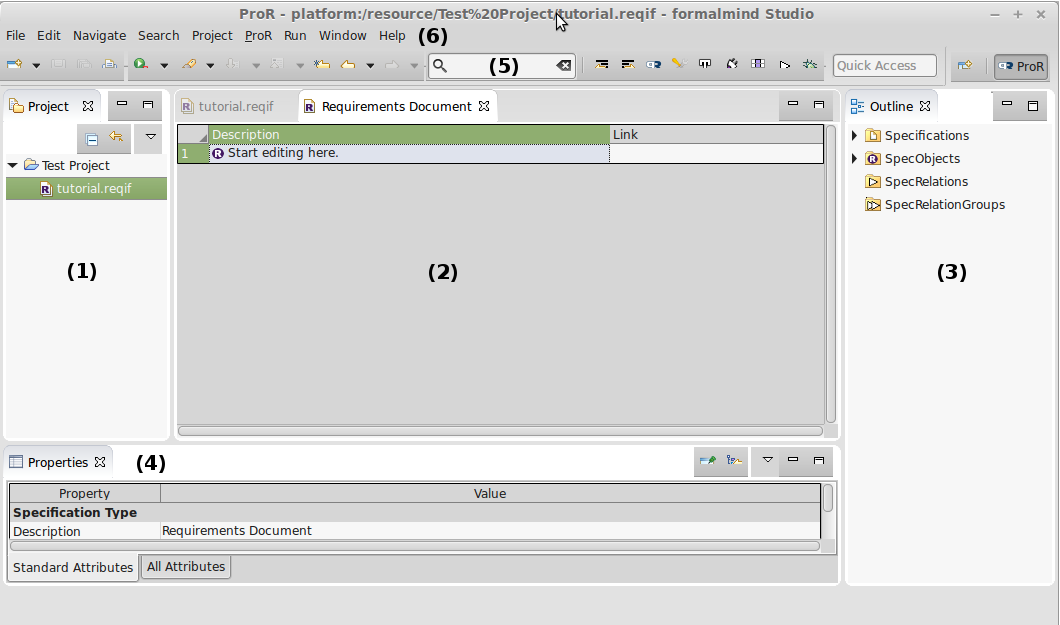
\includegraphics[width=\linewidth]{../rmf-images/Screenshot_intro.png}
  \caption{The \pror{} user interface}
  \label{fig:user_interface_overview}
\end{figure}

\paragraph{(1)} The \menu{Project Explorer} shows a hierarchical listing of the project and the associated models.

\paragraph{(2)} The editor area shows two kinds of editors.  First, each ReqIF file has a \menu{ReqIF Editor} that shows basic information about the mode.  In addition, \menu{Specification Editors} can be opened for each Specification.

\paragraph{(3)} The \menu{Outline View} has four folders that show the content of the selected model:

\begin{description}

\item[Specifications] shows the Specifications in the ReqIF model.  You can
  expand the tree to expose the hierarchy of SpecObjects in each Specification.
\item[SpecObjects] shows all SpecObjects in the ReqIF model as a flat list.
  Keep in mind that SpecObjects in Specifications are references.  In
  contrast, this folder shows all SpecObjects created for the ReqIF model, whether or not they are referenced.
\item[SpecRelations] shows all SpecRelations in the ReqIF as a flat list.
\item[SpecRelationsGroups] represents an optional mechanism for grouping SpecRelations between two specific specifications.
\end{description}

\paragraph{(4)} The properties of a selected Element are shown in the \menu{Properties View}.  It has two tabs, one for \menu{Standard Attributes} and one for \menu{All Attributes}.

\paragraph{(5)} Above the main working windows is the tool bar, which may change according to which editor is active.

\paragraph{(6)} The menu bar provides access to all Eclipse and \pror{} features.

% -----------------------------------------------------------------------------------
\subsection{Editors and Views}
\label{sec:editorsviews}
\index{editor}
\index{view}
% -----------------------------------------------------------------------------------

The Eclipse user interface consists of \term{Views} and \term{Editors}.  Views change their content according to the current selection and are not savable.  Editors are typically associated with a resource (e.g. a file) and can be saved.  The editors' selection can determine what is shown in the Views.  For instance, the \menu{Properties View} typically shows details about the element selected in the \menu{Specification Editor}.

You can browse through the available Views and open them via \menu{Window | Show Views...}, resulting in a menu similar to the one shown in Figure~\ref{fig:Views}.

\begin{figure}
\centering
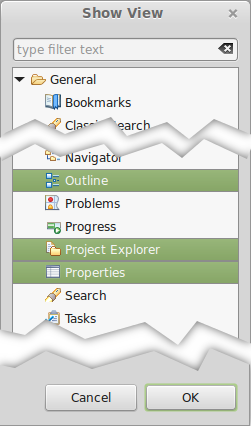
\includegraphics[width=.3\textwidth]{../rmf-images/views_highlighted.png}
\caption{Views.}
\label{fig:Views}
\end{figure}

Upon opening a ReqIF model, the editor opens providing an overview of the model.  In essence what you are seeing is the Eclipse Workbench, with several modifications.  Here you will find a quick overview of each component.  A more detailed description of the Workbench can be found in 
\eclipsehelp{org.eclipse.platform.doc.user/reference/ref-43.htm}{Eclipse's Workbench User Guide}.

\begin{info}
  There may be more than one editor for a given file type.  To pick a specific one, right-click the file and select \menu{Open With...}, which will give you the list of installed editors.  In particular, the \menu{ReqIF Studio Main Editor} from Formal Mind is more powerful than the stock editor (see Section~\ref{sec:StudioSpecEditor}).
\end{info}

A model contains any number of Specifications, and the details of each Specification can be inspected individually.  The windows in which all relevant information appears are called \term{views}.  At your disposal are many views with productivity, debugging, help and team resources.  We will be focusing only on the views relevant to \pror{}.

% -----------------------------------------------------------------------------------
\subsection{ReqIF Editor}
\label{sec:reqif-editor}
\index{editor!ReqIF}
\index{ReqIF editor}
% -----------------------------------------------------------------------------------

The \menu{ReqIF Editor} is the first editor that opens when opening a ReqIF file. It is shown in Figure~\ref{fig:reqif-editor}.

\begin{figure}
\centering
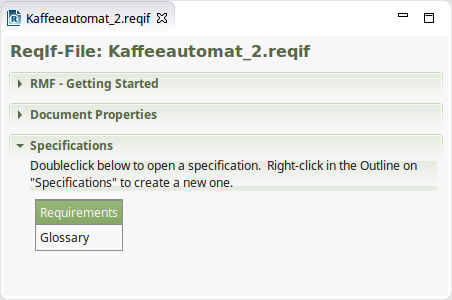
\includegraphics[width=.7\textwidth]{../rmf-images/reqif-editor.png}
\caption{ReqIF Editor}
\label{fig:reqif-editor}
\end{figure}

The \menu{ReqIF Editor} lists all Specifications, which can be opened by double-clicking. 

\begin{info}
If only one Specification is contained in the ReqIF file, it is opened automatically in a \menu{Specification Editor}.
\end{info}

Further, there are a few sections that are collapsed by default:

\begin{description}
\item[RMF -- Getting Started.] This section contains some basic information for new users.
\item[Document Properties.] This section show the embedded metadata. Some of it can be edited, some elements are read-only, as they are set by the tool.
\end{description}

% -----------------------------------------------------------------------------------
\subsection{Errors in ReqIF Editor}
\label{sec:errors-reqif-editor}
\index{errors}
\index{problems}
% -----------------------------------------------------------------------------------

If a ReqIF file is invalid, then \pror{} makes an attempt to recover. If this succeeds, then the \menu{ReqIF Editor} will show two tabs, as shown in Figure~\ref{fig:error-editor}. 

\begin{figure}
\centering
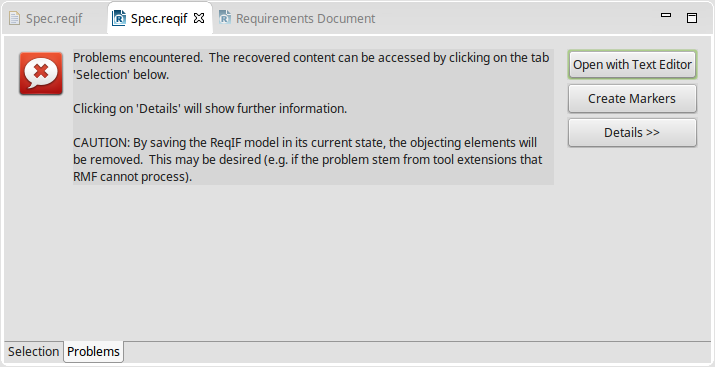
\includegraphics[width=.7\textwidth]{../rmf-images/error-editor.png}
\caption{ReqIF Editor with an active error tab}
\label{fig:error-editor}
\end{figure}

On the bottom, the editor now has two tabs, labeled \menu{Selection} and \menu{Problems}. The \menu{Problems} tab has three options:

\begin{description}
\item[Open with Text Editor.] This button will open the raw XML in a text editor. It is recommended to press \menu{Create Markers} first.
\item[Create Markers.]  This button will create error markers. This helps to pinpoint the problematic XML in the text editor.
\item[Details.] This will open an area showing the error tree. This information will also be shown in the \menu{Problem View}.
\end{description}

The \menu{Selection} tab shows the recovered ReqIF. Depending on the reason for the error condition, most or even all of the ReqIF is still there.

Saving the file will remove all problematic elements.

\begin{info}
A problematic ReqIF file can be fixed by simply by saving the ReqIF file again. It is recommended to inspect hte recovered ReqIF first, and to make a backup.
\end{info}

% -----------------------------------------------------------------------------------
\subsection{RMF Specification Editor}
\label{sec:spec-editor}
% -----------------------------------------------------------------------------------

\begin{figure}
  \centering
  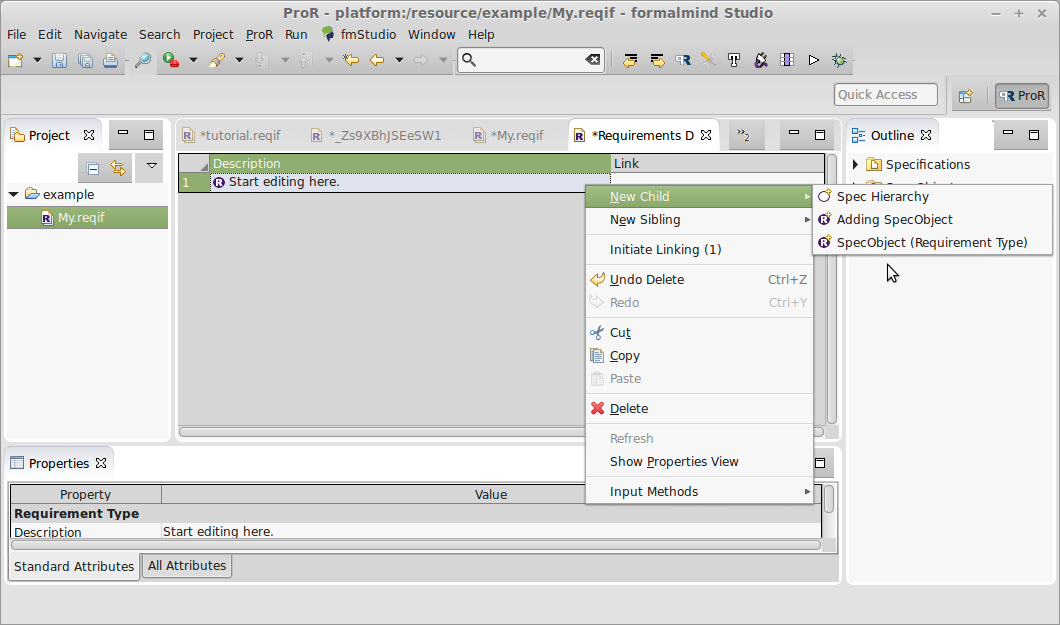
\includegraphics[width=\linewidth]{../rmf-images/default_spec_view.png}
  \caption{Specification Editor with the context menu open for creating a new child element}
  \label{fig:default specification editor}
\end{figure}

The Specification Editor shows the SpecObjects of a Specification, arranged in a grid view.  The hierarchy is shown via the indent of the first column, as well as through the numbering in the row header.

The columns show the Attributes with the names that match the column names (as shown in the header).  The columns can be resized by dragging.  Other operations, in particular reordering, adding and deleting columns are done via the \menu{Column Dialog}, accessible via \menu{Studio | Column Configuration } or the toolbar 
\includegraphics[height=0.8em]{../rmf-images/icons/full/obj16/Column.png}. 

The leftmost column shows the hierarchy and carries an icon.  The icon indicates whether it is a lone SpecHierarchy 
\includegraphics[height=0.8em]{../rmf-images/icons/full/obj16/spechierarchy.png} or a SpecObject 
\includegraphics[height=0.8em]{../rmf-images/icons/full/obj16/requirement.png}.

\begin{info}
Would you like to rearrange the columns?

In ReqIF Studio, you can simply drag the columns by grabbing them by their headers.

In Eclipse RMF, this does not work. Instead, use the following approach, which also works with ReqIF Studio:
In the top half of the \menu{Column Configurator} {
\includegraphics[scale=0.6]{../rmf-images/icons/full/obj16/Column.png}} window, a list of the exiting columns appear. Simply drag and drop them into the desired order. The changes appear in real time in the \menu{Specification Editor}. Close the window and the changes will be accepted.
\end{info}

Information can be entered either directly into the cell by double-clicking it or via the \menu{Properties View}.  While the Specification Editor only allows the editing of those attributes for which a column exists, the \menu{Properties View} will always show all attributes.

\begin{figure}
  \centering
  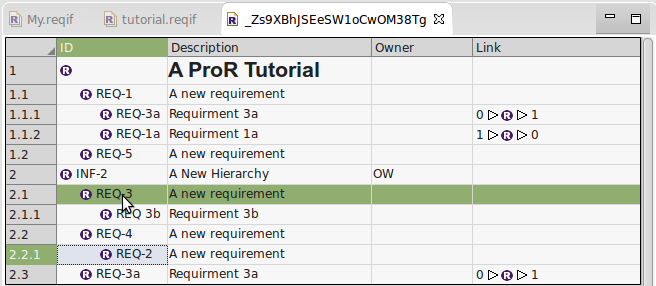
\includegraphics[width=0.8\linewidth]{../rmf-images/hierarchy_step_1.png}
  \caption{Click on a requirement and drag onto target parent.}
  \label{fig:hierarchy_step_1}
\end{figure}
\begin{figure}
  \centering
  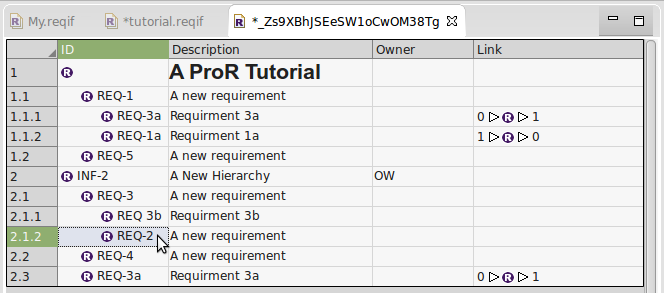
\includegraphics[width=0.8\linewidth]{../rmf-images/hierarchy_step_2.png}
  \caption{Result: The requirement is now a child of the chosen parent.}
  \label{fig:hierarchy_step_2}
\end{figure}

The SpecObjects can be reordered via drag and drop.  To move an existing SpecObject into the position of parent or child of another existing SpecObject, simply drag the child directly \textit{onto the target SpecObject}, as shown in Figure~\ref{fig:hierarchy_step_1}. The result is shown in Figure~\ref{fig:hierarchy_step_2}. 

Alternatively, as you drag the SpecObject \textit{onto the line below or above} the level you would like to move it to, it will become a sibling rather than a child of the SpecObject.  This is shown in Figure~\ref{fig:hierarchy_step_3}, with the resulting ordering shown in Figure~\ref{fig:hierarchy_step_4}.

\begin{figure}
  \centering
  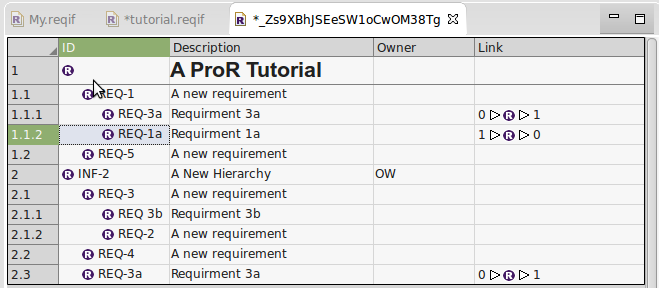
\includegraphics[width=0.8\linewidth]{../rmf-images/hierarchy_step_3.png}
  \caption{Click on a requirement and drag onto the line (bolded) below or above target sibling.}
  \label{fig:hierarchy_step_3}
\end{figure}
\begin{figure}
  \centering
  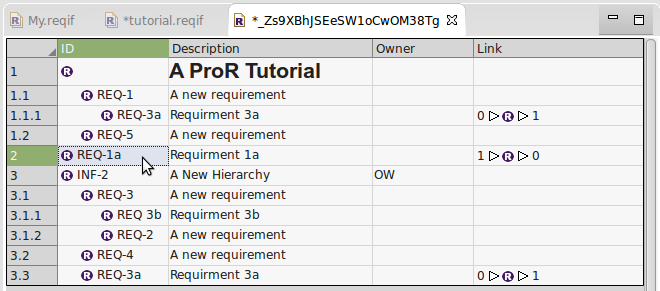
\includegraphics[width=0.8\linewidth]{../rmf-images/hierarchy_step_4.png}
  \caption{Result: The requirement is now a sibling of the chosen requirement.}
  \label{fig:hierarchy_step_4}
\end{figure}

To duplicate a SpecObject, simply copy and paste it into the required position. The copying, cutting and pasting functions are accessible through the traditional dropdown menu, by right-clicking on a desired cell or the corresponding keyboard shortcut.

By right clicking on any cell, you have a few options at your disposal. Outside of the usual \menu{Undo}, \menu{Cut}, \menu{Copy}, \menu{Paste} and \menu{Delete}, commands, the following are also available:

\begin{description}
\item
  [New Child.] A new SpecObject will be created as a child element.
\item
  [New Sibling.] A new SpecObject will be created as a sibling element.
\item
  [Initiate Linking.] This is the option to create a link between requirements. Once a link is initiated and then by right clicking a target selection, the options to complete the links either to or from a selection will appear. By default, the links are illustrated in the \menu{Link} column to the right. 
\item
  [Show Properties View.] Opens the \menu{Properties View}, where the selected element can be inspected and edited.
\end{description}

% -----------------------------------------------------------------------------------
\subsection{Project Explorer View}\index{project explorer}
\label{sec:project-explorer}
% -----------------------------------------------------------------------------------

The \menu{Project Explorer View} is by default on the left side of the main window. Here you can inspect files and models associated with any project. If for some reason the Project Explorer View does not appear, Navigate to \menu{Window | Show View | Other | Project Explorer View}.

In the main area  of this viewer is a hierarchical listing of the project and it's components. Use the black arrow to the left to collapse or display the project's contents. Below the view's title and to the right are the options to collapse the project folder and link the project with the editor. To the right of these options is another dropdown menu.

This view is covered in more detail by the \eclipsehelp{/topic/org.eclipse.platform.doc.user/reference/ref-27.htm}{Eclipse documentation}.

% -----------------------------------------------------------------------------------
\subsection{ReqIF Validation}\index{validation}\index{ReqIF validation}
\label{sec:reqif-validation}
% -----------------------------------------------------------------------------------

ReqIF is spreading, and partners start handing .reqif and .reqifz files back and forth.  But chances are that the first import of such a file will fail.  What is the problem? Consequent, the free ReqIF-Validator may provide the answer.

The validation results are shown in the Eclipse Problem View.  In addition, it is possible to open the ReqIF file in question in a text editor and to generate error markers, as shown in Figure~\ref{fig:error-marker}.

\begin{info}
In addition to the validator that is built into the tool, there is also a command line version available, which can be downloaded for free from \url{https://reqif.academy}.
\end{info}

\begin{figure}
\centering     
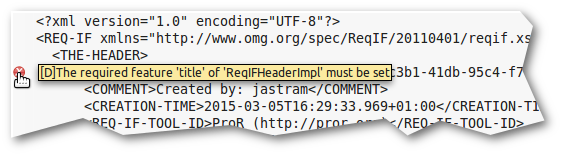
\includegraphics[width=\linewidth]{../rmf-images/error-marker.png}
\caption{Error Markers generated by Consequent}
\label{fig:error-marker}
\end{figure}

You can validate a ReqIF file as follows:

\begin{itemize}
\item    Right-Click the file to be validated in the Project Explorer (no need to open the file)
\item    Select \menu{Validate | Consequent ReqIF Validation}
\item    A dialog indicates the completion of the validation, which is shown in the Problem View.
\item    If the Problem View is not visible, open it by hand via \menu{Window | Show View | Other... | General | Problems}
\item    To see the error in the file, you must open it in a text editor as follows:
\begin{itemize}
\item        Right-Click the file in the Project Explorer
\item        Select Open With | Text Editor
\item        Errors are shown with an icon in the left margin (hovering over the error reveals the problem) – see screenshot below
\item        For errors with line numbers, it is possible to double click on an error in the Problem View to jump to the corresponding position in the Text Editor
\end{itemize}

\item    Error markers do not reset automatically. Re-run the validation to update them. You can manually clear error markes (e.g. for files that do not exist any more) by right-clicking on an element in the Problem View and selecting Delete.
\end{itemize}

\subsubsection{Validation Rules}

You can access and individually disable the validation rules via \menu{Window | Preferences | Model Validation | Constraints}.

\begin{info}
A printable version of the validation rules can retrieved from the build server at
\url{http://hudson.eclipse.org/rmf/job/rmf.develop.mars/ws/org.eclipse.rmf.reqif10.constraints/plugin.xml}
\end{info}

\subsubsection{Consequent Acknowledgement}

Consequent is part of the open source Eclipse project and was financed by the ProStep ReqIF Implementor Forum.

% ===================================================================================
\section{Configuration and Preferences}
\label{sec:config-preferences}
% ===================================================================================

Both the current model, as well as \pror{} as a whole, can be configured and customized extensively.

% -----------------------------------------------------------------------------------
\subsection{Global Preferences}
\index{preferences}
\index{validation!on save}
\index{Consequent!validate on save}
\label{sec:global-prefs}
% -----------------------------------------------------------------------------------

The application-wide settings of \pror{} are accessed via \menu{Window | Preferences | ReqIF}, as shown in Figure~\ref{fig:rmf-preferences}.  Configuration elements are:

\begin{figure}
\centering     
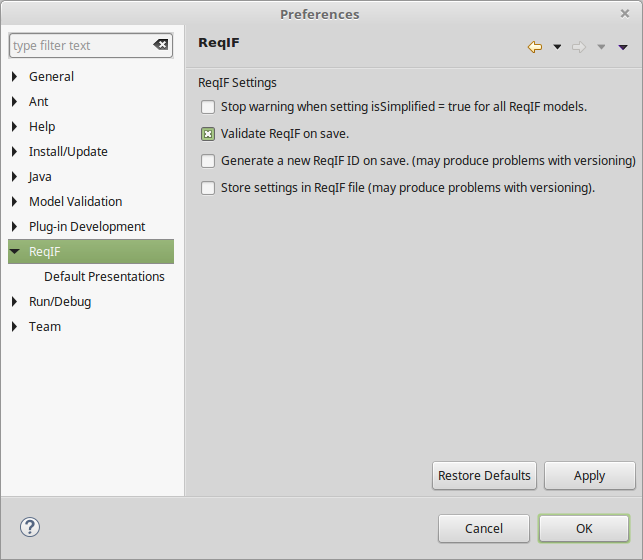
\includegraphics[width=0.8\linewidth]{../rmf-images/rmf-preferences.png}
\caption{The Global Preferences, with a sub-page for Defaultt Presentations.}
\label{fig:rmf-preferences}
\end{figure}

\begin{description}
\item[Warning regarding isSimplified.] This allows a warning to be issued if the content of a rich text attribute has the ``isSimplified'' flag set, which is defined by the ReqIF standard. This is relevant for tools that are not capable of editing rich text, without converting it to plain text first. This is only relevant when not using the rich text editor from ReqIF Studio. It is also possible to disable the rich text editor via the \menu{Default Presentations} sub-page.
\item[Validate ReqIF on save.] When checked, Consequent, the ReqIF validator, is automatically run on saving, with the validation result shown in the \menu{Problem View}. For larger files, this can take a while. If disabled, it is recommended to run the validator manually once in a while (via the ReqIF file's context menu).
\item[Generate a new ReqIF ID on save.] Every time a ReqIF file changes, its ID should change. However, in a team environment, this can create problems: When two people work on the same file, there would always be a conflict, as both IDs would have changed. Therefore, this can be disabled. If disabled, then the ReqIF Exporter (Section~\ref{sec:export}) should always be used, as it can change the ID upon export.
\item[Store Settings in ReqIF file.] The configuration of the columns of a Specification can be stored inside the ReqIF file. This is useful when the recipient of a ReqIF file should have a certain configuration of the columns. However, this can create problems in a team environment, as changes in the column configuration can create conflicts. If unchecked, this information will be stored in a separate file, which has the same name as the ReqIF file, but ends in \menu{.rmf}. That file should not be put under version control.

\end{description}

\subsubsection{Default Presentations}

\pror{} has basic cell editors for each ReqIF \term{Datatypes}.  But it is possible to install new editors with better or different capabilities.  With this setting, Presentations can be selected to handle certain Datatypes by default. It is not recommended to change the settings here.

\begin{warning}
There is no validation taking place in this dialog, use at your own risk.
\end{warning}

By default, the setting for each Datatype is ¸¸None''. This means that the build-in handler is used. However, Presentations can signal that they can improve the handling of the Datatype and install themselves as the handler automatically.

The use of the built-in handler can be forced by selecting ``Use Build-in''.

For each of the seven Datatypes, there is a dropdown listing all installed Presentations. Note that \textbf{all} are listed, there is no checking on whether a Presentation can actually handle the given datatype. A Presentation can be actively selected, then the use if it is fixed.

\begin{info}
\index{XHTML}
Particularly popular is the free Presentation from Essentials for handling XHTML.  The standard editor from RMF converts rich text to plain text.  The rich text Presentation is preinstalled with ReqIF Studio and will register itself automatically as the handler for XHTML.
\end{info}

% -----------------------------------------------------------------------------------
\subsection{General Configuration}
\index{configuration!general}
\label{sec:general_configuration}
% -----------------------------------------------------------------------------------

This configuration is accessed either via \menu{Studio | General Configuration}, or
via the 
\includegraphics[height=0.8em]{../rmf-images/ReqIFUIToolExtension.png} button on the toolbar.

Currently, there is only one configuration element: \menu{Label Configuration}.

% -----------------------------------------------------------------------------------
\subsubsection{Label Configuration}
\index{label configuration}
\index{configuration!label}
\label{sec:label-configuration}
% -----------------------------------------------------------------------------------

The \menu{Label Configuration} is used to determine what to use for the text labels of elements
in places, where a shorthand is needed.  Examples are elements in the \menu{Outline View} or the link targets in the \menu{Link} column.

\begin{figure}
\centering     
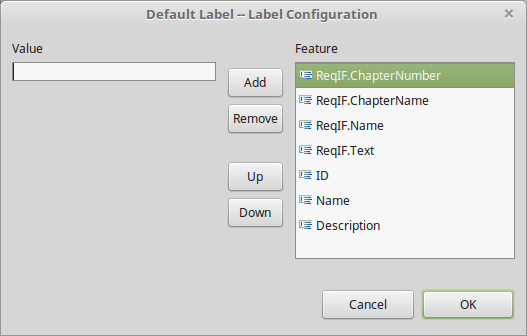
\includegraphics[width=0.8\linewidth]{../rmf-images/label-configuration.png}
\caption{The Label Configuration consists of a list of attribute names. To find the label for a SpecElement, the list is scanned from top to bottom to find a matching attribute, which is then used as the label. If none is found, the internal ID is used.}
\label{fig:label-configuration}
\end{figure}

\pror{} will determine the label by looking at the \menu{Label Configuration}, which is a list of text strings (see Figure~\ref{fig:label-configuration}.
To identify the label of an element, \pror{} will go through the list, top to bottom.  If the element has an attribute with a matching name, that attribute value is used as the label.

If none is found, then the element's internal ID is displayed.

Figure~\ref{fig:label-configuration} provides an example. For instance, the label for a SpecObject in the \menu{Outline View} is found by first looking for an attribute named ``ReqIF.ChapterNumber''. If one is found, it is used as the label. If not, \pror{} looks for ``ReqIF.ChapterName'', and so on, until one is found. If none is found, the internal ID is used.

To configure, select \menu{Label Configuration} in the top pane of the dialog.  On the bottom pane, you see the \menu{Default Label} property.  Doubleclick the value (on the right), then click on the ellipses (...) to open the configuration dialog.  Under \menu{Feature}, you will see the list of attribute names that will be used for the label, if found.

Use the \menu{Add} and \menu{Remove} buttons to add more attribute names to be searched for.  The
search order can be adjusted with \menu{Up} and \menu{Down}.

\begin{info}
It is good practice to use the ID Presentation (\ref{sec:id_presentation}) to generate
user-friendly IDs, and to use these as the first match for a label.  As IDs are unique, you'll always
have a unique identifier that is typically also used for communication.
\end{info}

% -----------------------------------------------------------------------------------
\subsection{Datatype Configuration}
\index{configuration!datatype}
\index{datatype configuration}
\label{sec:datatype_configuration}
% -----------------------------------------------------------------------------------

\begin{figure}
\centering     
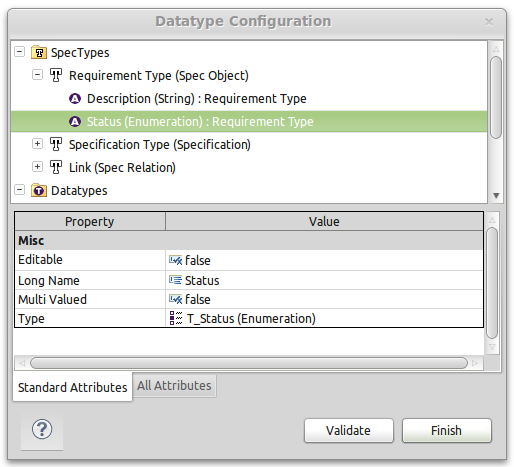
\includegraphics[width=0.8\linewidth]{../rmf-images/pror_datatype_configuration.png}
\caption{Datatype Configuration Dialog}      
\label{fig:DatatypeConfig}
\end{figure}

This configuration is opened via \menu{Studio | Datatype Configuration...}

The dialog shows two folders, one for SpecTypes and one for Datatypes.
SpecTypes are created for typing elements that have attributes
(SpecObjects, Specifications, SpecRelations).  New SpecTypes can be
created by right-clicking on the folder and selecting \menu{New Child}.
Through the same mechanism, attribute definitions can be added to a
SpecType.  Attribute definitions are typed.  Selecting an element shows
its properties in the lower pane, where it can be configured.

Attributes must have a name and a Datatype.  Some Attributes
allow further customization.  The Datatype is selected from a
dropdown.  New Datatypes can be created by right-clicking on the folder
\menu{Datatypes} and selecting \menu{New Child}.  Again, selecting a Datatype
shows its properties in the lower pane, where it can be configured.  A
Datatype should have at least the \menu{long name} property set.

As an example, consider the Datatype Configuration shown in Figure~\ref{fig:DatatypeConfig}.
The SpecType for ``Requirements Type,'' which is applicable to
SpecObjects, is expanded.  The SpecType has two Attributes,
``Description'' (String) and ``Status'' (Enumeration).  Status is
selected, and in the pane below the mandatory values, \menu{Long Name} and
\menu{Type} have been set.  Further customization of the attribute is
possible, e.g.  by converting it to a multi-valued Attribute by setting
the corresponding flag to \menu{true}.

\subsubsection{Enumeration Datatypes}

\begin{figure}
\centering      
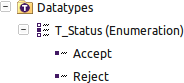
\includegraphics[width=0.3\linewidth]{../rmf-images/rmf_enumeration.png}
\caption{Enumerations}      
\label{fig:Enumerations}
\end{figure}

An Enumeration Datatype must have enumeration values.  These are created
by right-clicking the Enumeration Datatype and selecting \menu{New Child |Enum Value}.  You may have to unfold the enum value to select it, so that you can provide it with a \menu{Long Name}.  Figure~\ref{fig:Enumerations} shows a correctly configured Enumeration Datatype.

% -----------------------------------------------------------------------------------
\subsection{Presentation Configuration}\index{configuration!presentation}
\label{sec:presentation_configuration}
% -----------------------------------------------------------------------------------

Presentations are software components that extend the functionality of \pror{}.  Chapter~\ref{sec:presentations} is dedicated to Presentations.

% -----------------------------------------------------------------------------------
\subsection{Column Configuration}\index{configuration!column}
\label{sec:column_configuration}
% -----------------------------------------------------------------------------------

This configuration is specific to the Specification Editor.

The Column Configuration Dialog configures the Columns of a
Specification.  Columns are identified by name.  The width of the column
can be adjusted directly by dragging the column separator in the table
header.

If the SpecObject has an attribute where the name of the attribute
matches the name of the column, then that attribute is shown in that
column.

% ===================================================================================
\section{Access Control}
\index{access control}
\index{permissions}
\index{read-only}
\label{sec:access-control}
% ===================================================================================

The ReqIF standard provides a flag for marking certain elements as read-only.  This flag is accessible through the \menu{Properties View} by selecting the tab \menu{All Attributes}.  However, this flag is not honored in the user interface: even if an element is marked as read-only, it is normally writable.  We may implement this in the future.

\begin{warning}
Access Control is a ReqIF feature designed for data exchange.  As \pror{} uses ReqIF as a data model (and not as an exchange format), access information is only stored, but not used for managing access.
\end{warning}

% ===================================================================================
\section{Import and Export}
\label{sec:import-export}
% ===================================================================================

Importers and Exporters are accessed via \menu{File | Import...} and \menu{File | Export...}.  The corresponding dialogs will show generic Importers and Exporters, as well as specific ones.  The specific ones are in a folder called \menu{\pror{} (ReqIF)}.

This section also lists Importers and Exporters from third parties. Note that not all third-party Importers and Exporters may be listed here.

% -----------------------------------------------------------------------------------
\subsection{Import}
\index{import}
\label{sec:import}% -----------------------------------------------------------------------------------

The following importers exist:

\begin{description}
\item[ReqIFz Import.] This standard importer takes ReqIF archive (.reqifz) and imports it as an Eclipse project.

\item[CSV.] This standard importer takes comma-separated data and imports it into an existing ReqIF model.  It is described further below.

\item[Axiom.] This commercial importer supports the selective merging of exchange data with an existing ReqIF model.  It is described in detail in Section~\ref{sec:axiom}.

More information at the \href{https://reqif.academy}{ReqIF Academy}.

\end{description}

% -----------------------------------------------------------------------------------
\subsubsection{CSV Import}
\index{import!CSV}
\label{sec:csv-import}
% -----------------------------------------------------------------------------------

The CSV import adds the content from a comma-separated file into an existing specification.  Therefore, you first need to create a ReqIF model.  Once this is done, the importer is used as follows:

\begin{warning}
The importer will create new SpecTypes, Attributes and Datatypes.  Your existing types will not be reused!  We recommend to clean up the datatypes after the import.
\end{warning}

\begin{figure}
  \centering
  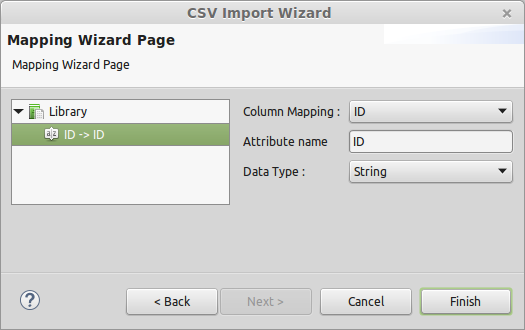
\includegraphics[width=0.8\textwidth]{../rmf-images/CSV_import.png}
  \caption{A complete mapping for a CSV import}
  \label{fig:csv}
\end{figure}

\begin{itemize}
\item Initiate the importer via \menu{File | Import... | ReqIF | CSV}.  

\item On the first dialog page, you need to select the source file containing the CSV data. The dialog defaults to comma-separated data, but other separators can be chosen as well.

\item A checkbox allows to indicated whether the file contains a header row.  If it is checked, the first row will be interpreted as the labels for the columns in the file.

\item Last, the destination model has to be chosen.  After this, the \menu{next} button is enabled.  

\item On the next page, the columns have to be mapped.  Initially, there is just a single element, \menu{Library}.

\item Right-click \menu{Library} to open the context menu that allows you to add a new mapping.  There are four options.  They all do the same, but the first three prepopulate the attribute name with a sensible value.

\item You need to create a mapping for each column that you would like to import.  A mapping consists of three elements:

\begin{description}
\item[Column Mapping.] Select the column from the CSV file.  The column headings are shown if the checkbox was selected on the previous page, otherwise just the column numbers.
\item[Attribute Name.] The name for the Attribute in the resulting ReqIF model.
\item[Data Type.] The datatype of the resulting attribute.  The safest option is \menu{String}, for other datatypes, a conversation attempt is made.
\end{description}

\item You do not need to create a mapping for all columns.  Figure\ref{fig:csv} shows the importer dialog with one complete mapping.

\item  Once all mappings are complete, hitting finish will complete the import.

\end{itemize}

You can read more in the \href{http://formalmind.com/blog/new-stuff-new-committer-new-product-new-importer-new-release}{Formal Mind Blog}.

% -----------------------------------------------------------------------------------
\subsection{Export}
\index{export}
\label{sec:export}
% -----------------------------------------------------------------------------------

The following exporters exist:

\begin{description}
\item[ReqIFz Export.] This standard exporter takes an Eclipse project and produces a ReqIF archive (.reqifz).

\item[Axiom.] This commercial exporter supports the selective exporting of exchange data for supplier communication.  More information at the \href{https://reqif.academy}{ReqIF Academy}.

\item[HTML.] The HTML export is not a ``real'' export, as it is accessed differently.  It produces an HTML view from an open Specification.  To use it, you need to have a Specification Editor open.  Then select \menu{File | Print...}.
\end{description}

% ===================================================================================
\section{Searching and Filtering}
\label{sec:search}
\index{search}
% ===================================================================================

\pror{} has three search interfaces.  Each has a different focus:

\begin{description}
\item[Quicksearch (Section~\ref{sec:quicksearch}).] This interface allows search-as-you-type in the open editor.  It is useful for quickly finding the right row in a specification, but just performs a simple text search on all attributes.
\item[ReqIF Search (Section~\ref{sec:reqif_search}).] This interface allow the user-friendly construction of attribute-specific searches within the current model.
\item[Raw Search (Section~\ref{sec:raw_search}).] This interface is powerful, but requires the queries to be constructed by hand.  It allows to fine-tune the search scope, including the search of the whole workspace.
\end{description}

Except the quicksearch, the results are shown in the \eclipsehelp{/topic/org.eclipse.platform.doc.user/gettingStarted/qs-36b.htm}{Eclipse Search Result View}.

% -----------------------------------------------------------------------------------
\subsection{Quicksearch}
\label{sec:quicksearch}
\index{search!quicksearch}
\index{quicksearch}
% -----------------------------------------------------------------------------------

This feature allows you to search-as-you-type within the open Specification.  The search box is embedded in the toolbar and only visible if a Specification Editor is open.

\begin{center}

\includegraphics[height=3em]{../rmf-images/quicksearch.png}
\end{center}

You can just begin typing in the box.  With every keystroke, the view will update and collapse those rows that do not match.  All attributes are searched.

% -----------------------------------------------------------------------------------
\subsection{ReqIF Search}
\label{sec:reqif-search}
% -----------------------------------------------------------------------------------

Searching is initiated via \menu{Search | Search... | ReqIF Search}, or via the search icon 
\includegraphics[height=1em]{../rmf-images/icons/full/obj16/search.png} on the toolbar.  This will present you the wizard shown in Figure~\ref{fig:reqif_search}.

\begin{info}
The search dialog shows several tabs on the top.  This handbook will cover ReqIF Search and ReqIF Search (Raw)---our ReqIF search tools.  

Depending on your Eclipse configuration, other search option may be shown and may still be useful.  For instance, the \eclipsehelp{/topic/org.eclipse.platform.doc.user/reference/ref-45.htm}{File Search} is useful for searching within all files, including .reqif files.
\end{info}

\begin{figure}
  \centering
  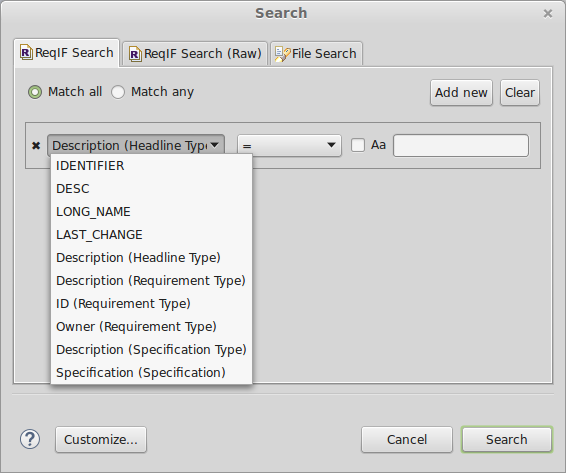
\includegraphics[width=0.8\textwidth]{../rmf-images/reqIF_search_1.png}
  \caption{ReqIF Search function with attribute dropdown menu}
  \label{fig:reqif_search}
\end{figure}
\label{sec:reqif_search}

% -----------------------------------------------------------------------------------
\subsubsection{Search Criteria}
% -----------------------------------------------------------------------------------

The ReqIF Search conditions consist of \textit{search criteria}, that are added by clicking on \menu{Add new}.  This creates a new criteria panel.  An arbitrary number of criteria can be defined.  Criteria can be removed by clicking on $\times$  on the left side of the panel, or by clicking \menu{clear} to remove all.

The radio button on top allows to either \menu{Match all} or \menu{match any} of the criteria.

Each criteria consists of three parts, \textit{attribute}, \textit{operator} and \textit{value}.  One such criteria is shown in Figure~\ref{fig:reqif_search}, with the attribute dropdown open.

\begin{description}
\item[Attribute.]  Choose an attribute (datatype) from the list.  The first four (IDENTIFIER, DESC, LONG\_NAME, and LA\-ST\-\_CHANGE) are ReqIF-internal attributes and are rarely of interest to normal users (see Section~\ref{sec:reqif_internal_attributes}).  The others attributes are taken directly from the document.  The more attributes you create, the longer the list will grow.  After you have chosen an attribute from the list, the rest of your choices (which are determined by the datatype of the attribute) are displayed.
\item[Operator.] The operator dropdown is specific to the selected attribute and is described for each type below.
\item[Value.] The value or values are specific to the operator and are also described below.
\end{description}

% -----------------------------------------------------------------------------------
\subsubsection{Operators for All Types}
% -----------------------------------------------------------------------------------

The following operators are available for all attributes, no matter what their type:

\begin{description}
\item[Equals (=).] For a match, the value must match \textit{exactly} as provided.  This implies that the attribute has actually been \textit{set}.  For instance, an empty string matches an empty string.  But it does not match if the value has not been set (i.e. if it is \textit{null}, in technical terms).
\item[Set.] For a match, the value must be set to any value. \textbf{Note:} A \term{default value} does not represent a match.
\item[Not set.] For a match, the value must not be set. \textbf{Note:} If the attribute in question does not exist, then there will not be a match either.  See example below.
\end{description}

\begin{example}
\textbf{Not Set Operator.}
Assume you receive a ReqIF model for review, with two SpecTypes, one called \textit{Information Type} which contains an attribute \textit{Description} and one called \textit{Requirement Type} which contains two attributes, \textit{Description} and \textit{Status}.  You are supposed to fill out the status for all requirements.

To find those that are still missing, you search for \menu{Status} \menu{not set}.  This will deliver all requirements for which no status has been set, even if there is a default value.
\end{example}

% -----------------------------------------------------------------------------------
\subsubsection{Operators for Plain and Rich Text}
% -----------------------------------------------------------------------------------

All text searches can be made case-sensitive by checking the corresponding checkbox \menu{Aa}.

The following operators are available for \textbf{plain text} attributes:

\begin{description}
\item[Not equals ($\neq$).] For a match, the value must not \textit{exactly} as provided.  If the attribute is not set, this constitutes a match.
\end{description}

The following operators are available for \textbf{plain text and rich text} (XHTML) attributes.

\begin{description}
\item[Contains.] For a match, the value must be a substring of the attribute.
\item[Contains not.] For a match, the value must not be a substring of the attribute. If the attribute is not set, this constitutes a match.
\item[Regexp.] The provided value will be interpreted as a \eclipsehelp{/topic/org.eclipse.platform.doc.isv/guide/st_text_types.htm?cp=2_0_3_9_1\#regex}{regular expression}.  Search will take place across line breaks.
\end{description}

\begin{info}
When searching rich text (XHTML), the invisible formatting will be included in the search, except for the \textit{regexp (plain)} operator described below.

Search will take place across line breaks.  But this is only relevant for Regexp search, where linebreaks can be matched explicitly (\menu{$\backslash$ n}) or as part of whitespace (\menu{$\backslash$ s}).
\end{info}

The following operators are available for \textbf{rich text} (XHTML) attributes.

\begin{description}
\item[Regexp (plain).] The provided value will be interpreted as a \eclipsehelp{/topic/org.eclipse.platform.doc.isv/guide/st_text_types.htm?cp=2_0_3_9_1\#regex}{regular expres\-sion}.  Search will take place against a version of the attribute value where the tags have been stripped out and been replaced by whitespace.
\end{description}

\begin{example}
\textbf{Searching XHTML.}  As XHTML contains invisible formatting tags, this should be taken into account when searching.  For instance, the search \menu{contains} \menu{formalmind.com} will find direct textual references to the domain, as well as hyperlinks. e.g. \texttt{<a href="http://for\-malmind.com">click</a>}.
\end{example}

% -----------------------------------------------------------------------------------
\subsubsection{Operators for Numbers (Integer and Real)}
% -----------------------------------------------------------------------------------

The interfaces for integer attributes and real attributes are identical, but the text boxes will only accept numbers of the appropriate type.

\begin{description}
\item[Not equal ($\neq$).] The provided value is not equal to the given number. This operator matches if the attribute has no value set.
\item[Between.] A match exists if the attribute value is between the given numbers, \textbf{including them}.
\item[Greater than ($>$).] A match exists if the attribute value is greater than the value, \textbf{excluding it}.
\item[Less than ($<$).] A match exists if the attribute value is less than the value, \textbf{excluding it}.
\end{description}

% -----------------------------------------------------------------------------------
\subsubsection{Operators for Dates}
% -----------------------------------------------------------------------------------

The granularity of the date criteria are one day, while \pror{} date stamps also include the time and have timezones.

\begin{warning}
\textbf{Timezones.} Dates in \pror{} have timezones.  The dates entered in the search interface assume the local time zone.  This can have implications if the values in the ReqIF model have been created by a user in a different time zone.  For example, consider a date has been written on ``Tuesday 23:00'' in the time zone of User~1.  But for User~2, it is already ``Wednesday 01:00''.  If User~1 would search for ``Tuesday'', there would be a match.  But for User~2, in a different time zone, not.
\end{warning}.

\begin{description}
\item[Equal ($=$).] The day matches, no matter what the time (but timezones apply).
\item[Not equal ($\neq$).] Any day except the given day, or not set.
\item[Between.] A match exists if the attribute value is between the given numbers, \textbf{including them}.
\item[Before.] A match exists if the attribute value is before the date, \textbf{excluding it} (i.e. before the time 00:00:00 on that date).
\item[After.] A match exists if the attribute value is after the date, \textbf{including it} (i.e. after the time 00:00:00 on that date).
\end{description}

% -----------------------------------------------------------------------------------
\subsubsection{Operators for Enumeration}
% -----------------------------------------------------------------------------------

While ReqIF enumerations may be single value or multi value, this distinction is immaterial for the search functionality.

\begin{description}
\item[Not equal ($\neq$).] Anything except an identical list will match.  \textbf{Note:} An empty list matches an unset attribute value.
\item[All.] All selected value must also be selected on the attribute (but the attribute may have more).
\item[Any.] For a match, at least one of the list values must also be set on the attribute.
\end{description}

% -----------------------------------------------------------------------------------
\subsubsection{Operators for Boolean}
% -----------------------------------------------------------------------------------

Only the standard operators (equals, set, not set) are available.

% -----------------------------------------------------------------------------------

% -----------------------------------------------------------------------------------
\subsubsection{Named Filters}
\label{sec:named-filters}
\index{filter}
\index{named filter}
% -----------------------------------------------------------------------------------

\pror{} provides a mechanism for saving filters, in order to allow reuse. Filters are saved within the project and can be applied to ReqIF files within a project.

\begin{warning}
Please note that applying filters to other ReqIF files within the same project will not
work. \pror{} will insert an empty filter, which need to be removed or reconstructed manually.
\end{warning}

By saving the filter for the project as a whole, they will survive if the file is renamed, as long as it stays in the project.

The filters are managed from the panel shown on the bottom of the filter panel, as shown in Figure~\ref{fig:named_filter}. To create a named filter, enter the name in the text box and press \menu{Save}.

\begin{figure}
  \centering
  
\includegraphics[width=0.8\textwidth]{../rmf-images/reqif_search_3.png}
  \caption{Controls for managing named filters}
  \label{fig:named_filter}
\end{figure}

The combo dropdown contains all named filters. After selecting them, a number of operations on the chosen filter are possible:

\begin{description}
\item[Load.] If the name in the combo does exist as a named filter, it can be loaded with \menu{Load}. The current filter settings will be lost.
\item[Save.] If the name in the combo does not exist as a named filter yet, \menu{Save} will create a new named filter.
\item[Update.] If the name in the combo does exist as a named filter, \menu{Update} will override it with the current filter configuration.
\item[Delete.] If the name in the combo does exist as a named filter, \menu{Delete} will remove it. This will not affect the current filter settings.
\end{description}

\begin{info}
Filters can be renamed in two steps: By saving an existing filter with a new name, and then deleting the old filter.
\end{info}

% -----------------------------------------------------------------------------------
\subsection{Raw ReqIF Search}
\label{sec:raw_search}
\index{search!raw ReqIF search}
\index{raw ReqIF search}
% -----------------------------------------------------------------------------------

The raw search feature has been described in the \href{http://formalmind.com/en/blog/formalmind-studio-pror-improvements-and-beta-program-about-start}{Formal Mind Blog}.



%%%%%%%%%%%%%%%%%%%%%%%%%%%%%%%%%%%%%%%%%%%%%%%%%%%%%%%%%%%%%%%%%%%%%%%%%%%%%%%%%%%%%%%%%

%%%%%%%%%%%%%%%%%%%%%%%%%%%%%%%%%%%%%%%%%%%%%%%%%%%%%%%%%%%%%%%%%%%%%%%%%%%%%%%%%%%%%%%%%
\chapter{Presentations}
\label{sec:presentations}
%*******************************************************************************
% Copyright (c) 2014 Formal Mind GmbH and others
% All rights reserved. This program and the accompanying materials
% are made available under the terms of the Eclipse Public License v1.0
% which accompanies this distribution, and is available at
% http://www.eclipse.org/legal/epl-v10.html
% 
% Contributors:
%     Michael Jastram - initial Copy
%     Maha Jastram - subsequent improvements
%******************************************************************************/

\pror{} has an extension mechanism that allows custom rendering, custom editing and automatic modifications to the requirements model. These extensions are called \term{presentations}.

Presentations can be created and configured via \menu{ProR | Presentation Configuration...} or the icon 
\includegraphics[height=1em]{../rmf-images/icons/full/obj16//ReqIFToolExtension.png} in the toolbar.  Launching it will show the dialog shown in Figure~\ref{fig:presentation-dialog}.  Initially, the dialog will be empty.  The dialog in the figure shows two presentation configurations.

Presentations are specific for a model, and its configuration is also stored in the requirements model.

\pror{} ships with a small set of standard presentations.  Additional presentations can be installed into \pror{}.

\begin{warning}
Note that presentations are specific to \pror{}, not to ReqIF.  This means that other tools will simply ignore presentations.  Also note that the behavior of the tool is unpredictable if a presentation used by a model is not installed in \pror{}.
\end{warning}

\begin{figure}
  \centering
  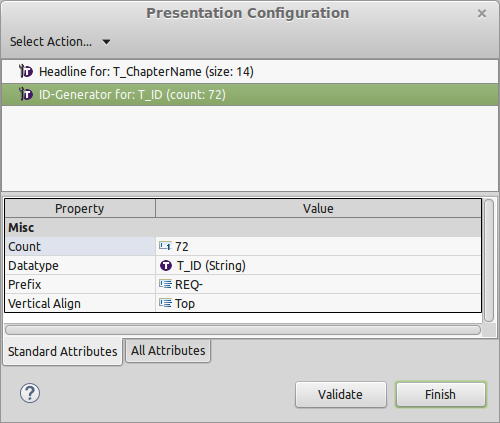
\includegraphics[width=0.8\textwidth]{../rmf-images/presentation-dialog.png}
  \caption{The presentation dialog with two configured presentations}
  \label{fig:presentation-dialog}
\end{figure}

% ===================================================================================
\section{Working with Presentations}
\index{presentation dialog}
% ===================================================================================

All presentations are configured in the same way.  To configure a presentation for the current model, first open the presentation configuration dialog as described above.

Initially, the dialog is empty.  You can add new presentations using the \menu{Select Action...} dropdown.  It will list all built-in and installed presentations.  Upon selecting an entry, it will be added to the list below.

\begin{info}It is possible (and often useful) to add the same presentation multiple times. For instance, one could add multiple ID generation presentations for different types of elements (with correspondingly different prefixes). 
\end{info}

Selecting a presentation in the upper pane will show its configuration parameters in the lower pane.  In Figure~\ref{fig:presentation-dialog}, the ID-Generator is selected, and the lower pane shows its four configuration parameters.

All presentations have a configuration parameter \menu{Datatype}.  Typically, the datatype determines whether a presentation is applied to an element or not.

\begin{info}
  If you want a presentation to be applied to a dedicated \term{Attribute} (rather than \term{Datatype}, then simply create a specific datatype for that attribute. And conversely, you can reuse a single presentation for multiple attributes by using the same datatype for all relevant Attributes.
\end{info}

The order of entries sometimes (but rarely) matters.  Presentations can be reordered using drag and drop.

Last, to delete a presentation, select \menu{Delete} from the context menu by right-clicking.

% ===================================================================================
\section{Default Datatype Handlers}
\index{presentations!default handlers}
\index{default handlers}
% ===================================================================================

Sometimes, it is desirable to use a presentation as the default for rendering (and editing) a specific datatype.  For example, the open source ProR can not render formatted (XHTML) text and instead shows a simplification in plain text.  But formalmind Studio offers the RTF presentation that allows rich rendering and editing.  Thus, it would be nice if XHTML datatypes would always be rendered using the RTF presentation, if installed.

This is possible.  And in fact, presentations can request to be used as default handlers.  If such a presentation is installed, it will automatically take over from the default.

Users can configure and override this.  To do so, go to \menu{Window | Preferences | ProR | Default Presentations}.  The resulting dialog is shown in Figure~\ref{fig:default-handlers}.

\begin{figure}
  \centering
  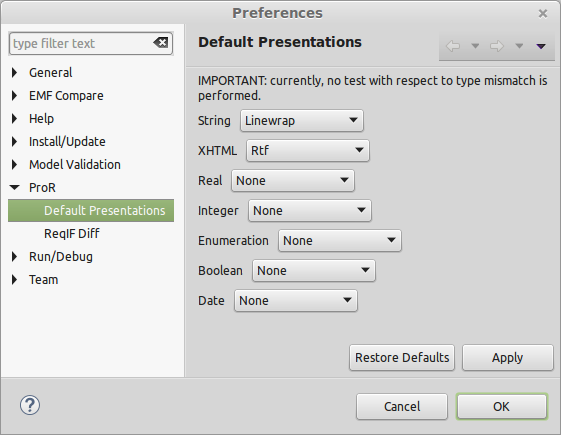
\includegraphics[width=0.8\textwidth]{../rmf-images/default-handlers.png}
  \caption{The preference dialog for handling default presentations}
  \label{fig:default-handlers}
\end{figure}

For each of the standard ReqIF datatypes, a handler can be chosen.  The default is \menu{none}.  The following entries are available:

\begin{description}
\item[None.] This is the default and implies that the build-in renderer is used.   Upon starting the tool, \pror{} will check whether a new presentation has been installed that requests to act as the default handler for that datatype.  If such a presentation is found, it will be set as the handler.
\item[Use Built-in.] This forces the built-in handler to be used.  Even if an installed presentation requests to be the handler, the built-in handler will continue to be used.
\item[List of installed presentations.] The remaining entries list all installed presentations.  Note that the dialog does not filter the matching types.  I.e. even though the RTF presentation is only applicable for XHTML, it is shown in the dropdown for all datatypes.
\end{description}

\begin{warning}
Please make sure that you only set datatype handlers of the correct type.  Also note that there is no access to the configuration parameters of default handlers. Therefore, this mechanism makes only sense for presentations that do not require any additional configuration.
\end{warning}

% ===================================================================================
\section{Built-in ProR Presentations}
\index{presentations!build-in ProR}
% ===================================================================================

The following presentations are part of the Eclipse RMF project and are therefore open source.

% -----------------------------------------------------------------------------------
\subsection{ID Generator Presentation}
\index{presentation!id generator}
\label{sec:id_presentation}
% -----------------------------------------------------------------------------------

This presentation automatically generates user-friendly IDs, consisting of a prefix and a number, e.g. ``REQ-12''. The configuration parameters are shown in Figure~\ref{fig:default-handlers}.

\begin{info}
Attributes to which this presentation applies are read-only and cannot be edited manually any more (as long as the presentation is active).
\end{info}

The parameters are:

\begin{description}
\item[Count.] The counter position. When a new ID is created, it will be incremented by one.  Changing it allows  the user to start or continue with a different number.
\item[Datatype.] The presentation will be applied to all attributes with this datatype.  Must by of type \term{String}.
\item[Prefix.] The prefix to the number.  Note that changing this will only modify newly created IDs, not those already generated.
\item[Vertical align.] Allows to adjust how the text shall be rendered in the cell.
\end{description}

\begin{warning}
Currently, the presentation does not check whether duplicate IDs exist!
\end{warning}

% -----------------------------------------------------------------------------------
\subsection{Headline Presentation}
\index{presentation!headline}
% -----------------------------------------------------------------------------------

This presentation renders the content of a cell boldface in a large font.  This can be useful if
you want to format text to stand out (e.g. a headline), without having to resort to XHTML.

The parameters are:

\begin{description}
\item[Datatype.] The presentation will be applied to all attributes with this datatype.  Must by of type \term{String}.
\item[Size.] The size of the text in point.
\end{description}

% -----------------------------------------------------------------------------------
\subsection{Linewrap}
\index{presentation!linewrap}
% -----------------------------------------------------------------------------------

This presentation wraps text at word boundaries, essentially what one would expect anyway.  The built-in renderer breaks the text anywhere, including in the middle of words.

This presentation is usually set as the default presentation.

\begin{info}
Regular users can just ignore this presentation.  It has been created for developers to understand the presentation mechanism.
\end{info}


%%%%%%%%%%%%%%%%%%%%%%%%%%%%%%%%%%%%%%%%%%%%%%%%%%%%%%%%%%%%%%%%%%%%%%%%%%%%%%%%%%%%%%%%%

%%%%%%%%%%%%%%%%%%%%%%%%%%%%%%%%%%%%%%%%%%%%%%%%%%%%%%%%%%%%%%%%%%%%%%%%%%%%%%%%%%%%%%%%%
\chapter{Style Guide}
\label{sec:styleguide}
%*******************************************************************************
% Copyright (c) 2014 Formal Mind GmbH and others
% All rights reserved. This program and the accompanying materials
% are made available under the terms of the Eclipse Public License v1.0
% which accompanies this distribution, and is available at
% http://www.eclipse.org/legal/epl-v10.html
% 
% Contributors:
%     Michael Jastram - initial Copy
%     Maha Jastram - susequent improvements
%******************************************************************************/

This simple guide is intended to explain the style used in this documentation.  We request that you follow it as closely as possible when creating content in order to maintain a clear, concise and easy to read body of work.

The documentation was created with and is maintained with \LaTeX.  That stands to reason that much of the formatting is software-dependent, leaving us to worry about more important things.  But that still leaves some decisions for us to make.  For example, alphabetization, certain punctuation, spelling and hyphenation of certain words, and the like will be accounted for here.

% ===================================================================================
\section{alphabetization}
% ===================================================================================

What should and should not be alphabetized:

\begin{itemize}

\item
  General terms such as ``requirements'' or ``specifations'' not used in a ProR or Eclipse specific manner are written in lower-case.
\item
  ProR- and Eclipse-specific terms shall be capitalized.  i.e., terms such as ``Eclipse Workbench,'' ``SpecObject,'' ``Editor,'' and ``Views'' are capitalized.

\end{itemize}

% ===================================================================================
\section{Punctuation}
% ===================================================================================

\begin{itemize}

\item
  \textbf{Mdashes} shall be used when needed—here is a perfect example—with no spaces.  
\item
  \textbf{Periods} will be followed by double-spaces.
\item
  When \textbf{Colons} are used to introduce a series of numbered items in a list, do not capitalize the first item after the colon (unless it's a proper noun) and seperate the list items with semi-colons, e.g.:
  There are three differences: (1) the first difference; (2) the second difference; and (3) the third difference.
  
\end{itemize}

% ===================================================================================
\section{Contributing}
% ===================================================================================

Documentation is one of those things that gets easily neglected in open source projects.  It is also one of the easiest for outsiders to contribute to.  The documentation is managed as Latex, which may scare some people.  But no worries, those who don't want to learn Latex don't have to.

There are broadly two ways for contributing to the documentation:

\begin{description}
  \item[File a bug.]  Visit the \href{https://bugs.eclipse.org/bugs/enter_bug.cgi?assigned_to=&blocked=&bug_severity=normal&bug_status=NEW&comment=&contenttypeentry=&contenttypemethod=autodetect&data=&dependson=&description=&flag_type-1=X&flag_type-11=X&flag_type-12=X&flag_type-2=X&flag_type-4=X&flag_type-6=X&flag_type-7=X&flag_type-8=X&form_name=enter_bug&keywords=&&op_sys=All&product=MDT.RMF&qa_contact=&rep_platform=All&short_desc=&version=unspecified}{RMF Bug Tracker}.  You can just point out a problem or request for improvement.  You can also provide some text to be added to the documentation (unformatted).  If you do, however, then you need to sign a Committer License Agreement (CLA)
  \item[Submit improved \LaTeX via Gerrit.]  If you are technically inclined (meaning that you know what \LaTeX and git are, and how to use them), then you can contribute via the Gerrit code review system, as described \href{https://wiki.eclipse.org/Gerrit}{at eclipse.org}.
\end{description}

\subsection{Gerrit for Contributions}

TODO - when done, update the parent section as well.

% ===================================================================================
\section{Licensed as EPL}
% ===================================================================================

This work is licensed under the Eclipse Public License.

% ===================================================================================
\section{Acknowledgements}
% ===================================================================================

Many parties were involved in the creation of RMF.  We would like to thank the core team that made it possible.

\begin{figure}[H]
  \centering
  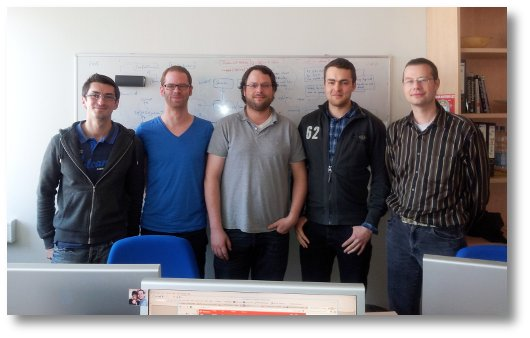
\includegraphics[width=\textwidth]{../rmf-images/2012_03_sprint_team.jpg}
  \caption{The RMF team during a Sprint in April 2012 in Düsseldorf, Germany
  (left to right) Lukas Ladenberger, Mark Brörkens, Ingo Weigelt, Said Salem, Michael Jastram}
  \label{fig:intro_core_team}
\end{figure}


The roots of this project were created by Andreas Graf, Michael Jastram and Nirmal Sasidharan, who joined together individual projects to create RMF.  Their efforts were financed by the research projects itea Verde and FP7 Deploy.  RMF was assembled at the Eclipse Foundation, where it has been active ever since.  Figure~\ref{fig:intro_core_team} shows four of the five RMF Committers at a joint coding session (missing is Andreas Graf).

%%%%%%%%%%%%%%%%%%%%%%%%%%%%%%%%%%%%%%%%%%%%%%%%%%%%%%%%%%%%%%%%%%%%%%%%%%%%%%%%%%%%%%%%%

%%%%%%%%%%%%%%%%%%%%%%%%%%%%%%%%%%%%%%%%%%%%%%%%%%%%%%%%%%%%%%%%%%%%%%%%%%%%%%%%%%%%%%%%%
\clearpage
\phantomsection
\addcontentsline{toc}{chapter}{Index} 
\printindex
%%%%%%%%%%%%%%%%%%%%%%%%%%%%%%%%%%%%%%%%%%%%%%%%%%%%%%%%%%%%%%%%%%%%%%%%%%%%%%%%%%%%%%%%%

\end{document}

